%-------------------------------------------------------------------------
%-------------------------------------------------------------------------
%-------------------------------------------------------------------------

\chapter{A Typology of Abstract Visualization Tasks}
\label{ch:typology}

%-------------------------------------------------------------------------
%-------------------------------------------------------------------------
%-------------------------------------------------------------------------

\begin{epigraph}
    \item \emph{``By thinking about visualization as a process instead of an outcome, we arm ourselves with an incredibly powerful thinking tool.''} ---~Jer Thorp in ``Visualization as process, not output''~\cite{Thorp2013} (\emph {Harvard Business Review}, April 3, 2013)
\end{epigraph}

\footnote{This chapter is a slightly modified version of our paper {\it A Multi-Level Typology of Abstract Visualization Tasks} by Matthew Brehmer and Tamara Munzner; in IEEE Transactions on Visualization and Computer Graphics (Proceedings of InfoVis 2013), 19(12), p. 2376--2385~\cite{Brehmer2013}. \url{http://dx.doi.org/10.1109/TVCG.2013.124}.}The considerable previous work characterizing visualization processes has focused on low-level tasks\index{task!low-level tasks} or interactions\index{interaction} and high-level tasks\index{task!high-level tasks}, leaving a gap between them that is not addressed\footnote{Referring to the examples cited in \autoref{intro:research-trajectory}, {\it finding an extreme value}~\cite{Amar2005} is an example of a low level of abstraction while {\it exploring}~\cite{Yi2007} or {\it integrating insights}~\cite{Springmeyer1992}\index{insight} are examples of a higher level of abstraction.}.
% RR: p. 3. "exploring [234] or integrating insights [188] are quite abstract". Do you really mean "abstract", or do you mean "vague"? (cf. discussion of "exploring" on p. 11.) Related to this: couldn't "finding an extreme value" be abstract?  If not, what do you mean by "abstraction"? Isn't this simply independence of the details of the task?
This gap leads to a lack of distinction between the ends\index{task!ends} and means\index{task!means} of a task\index{task}, limiting the potential for rigorous analysis.
We contribute a multi-level typology\index{task!task typology} of visualization tasks\index{task} to address this gap, distinguishing {\it why}\index{{\tt why}} and {\it how}\index{{\tt how}} a visualization task\index{task} is performed, as well as {\it what}\index{{\tt what}} the task\index{task} inputs\index{{\tt input}} and outputs\index{{\tt output}} are.
Our typology\index{task!task typology} allows complex tasks\index{task} to be expressed as sequences of interdependent tasks\index{task!task sequence}, resulting in concise and flexible descriptions for tasks\index{task} of varying complexity and scope.
It provides abstract rather than domain-specific descriptions of tasks\index{task}, so that useful comparisons can be made between visualization techniques or tools targeted at different application domains.
This descriptive power supports a level of analysis required for the generation of new designs, by guiding the translation of domain-specific problems into abstract tasks\index{task!task abstraction}, and for the qualitative evaluation\index{evaluation} of visualization tools or techniques.
We demonstrate the benefits of our approach in a detailed example, comparing task\index{task} descriptions from our typology\index{task!task typology} to those derived from related work.
We also discuss the similarities and differences between our typology\index{task!task typology} and over two dozen existing classifications and theoretical frameworks from several research communities, including visualization, \ac{HCI}\index{human-computer interaction (HCI)}, information retrieval\index{information retrieval}, communications\index{communications}, and cartography\index{cartography}.

%-------------------------------------------------------------------------
%-------------------------------------------------------------------------

\section{Motivation}
\label{typology:intro}

%-------------------------------------------------------------------------
%-------------------------------------------------------------------------

Consider a person who encounters a choropleth map\index{visual encoding!map!choropleth map} while reading a blog post in the aftermath of an American presidential election.
This particular map\index{visual encoding!map!choropleth map} is static and visually encodes\index{{\tt encode}} two attributes, candidate and margin of victory, encoded for each state using a bivariate colour mapping.
This person decides to compare\index{{\tt compare}} the election results of Texas to those of California, motivated not by an explicit need to generate\index{{\tt discover}} or verify\index{{\tt discover}} some hypothesis, nor by a need to present information to an audience, but rather by a casual interest in American politics and its two most populous states.
How might we describe this person's {\it task}\index{task} in an abstract rather than domain-specific way?

% \begin{figure}
%     \centering
%     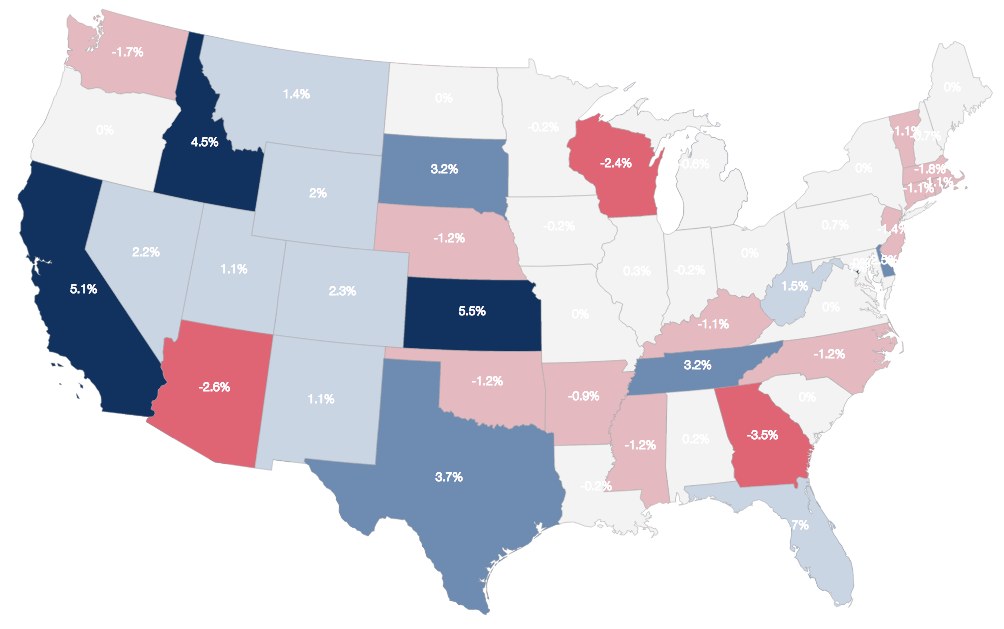
\includegraphics[width=0.8\textwidth]{figures/State_Choropleth.png}
%     \caption
%     [
%         A choropleth map.
%     ]
%     {
%         A choropleth map; \ccLogo~Deepthiyathiender, Wikimedia Commons (2015).
%     }
%     \label{typology:fig:chropleth}
% \end{figure}

According to Munzner's nested model\index{nested model (Munzner)} for visualization design and validation~\cite{Munzner2009}, abstract tasks\index{task!task abstraction} are domain- and interface-agnostic operations that people perform.
Disappointingly, there is little agreement as to the appropriate granularity of an abstract task\index{task!task abstraction} among the many existing classifications in the visualization, \ac{HCI}\index{human-computer interaction (HCI)}, cartography\index{cartography}, and information retrieval\index{information retrieval} literature~\cite{Amar2005,Amar2004,Andrienko2006,Buja1996,Card1999,Casner1991,Chi1998,Chuah1996,Dix1998,Gotz2008,Heer2012,Keim2002,Klein2006,Lee2006,Liu2010,Mullins1993,Pike2009,Pirolli2005,Raskin2000,Roth2012,Roth2013,Roth1990,Shneiderman1996,Spence2007,Springmeyer1992,Tweedie1997,Valiati2006,Ward2004,Wehrend1990,Yi2007,Zhou1998}.
One of the more frequently cited of these~\cite{Amar2005} would classify the above example as being a series of value retrieval tasks\index{task}.
This low-level\index{task!low-level tasks} characterization does not describe the person's context or motivation; nor does take into account prior experience and background knowledge.
For instance, a description of this task\index{task} might differ if the person was unfamiliar with American geography: the person must locate\index{{\tt locate}} and identify\index{{\tt identify}} these states before comparing\index{{\tt compare}} their values.
Conversely, high-level\index{task!high-level tasks} descriptions of exploratory data analysis and presentation emanating from the sensemaking\index{sensemaking} literature~\cite{Amar2004,Card1999,Klein2006,Pirolli2005} cannot aptly describe this person's task\index{task}.

The gap between low-level\index{task!low-level tasks} and high-level\index{task!high-level tasks} classification leaves us unable to abstractly describe tasks\index{task} in a useful way, even for the simple static choropleth map\index{visual encoding!map!choropleth map} in the above example.
This gap widens when interactive visualization techniques are considered, and the complexity of its usage is compounded over time.
We must move beyond describing a single task\index{task} in isolation, to a description that designates when one task\index{task} ends\index{task!ends} and another begins.
To close this gap, visualization tasks\index{task} must be describable in an abstract way across multiple levels.

The primary contribution of this chapter is a multi-level typology\index{task!task typology} of abstract visualization tasks\index{task} that unites the previously disconnected scopes of low-level\index{task!low-level tasks} and high-level\index{task!high-level tasks} classifications by proposing multiple levels of linkage between them.
Our typology\index{task!task typology} provides a powerful and flexible way to describe complex tasks\index{task} as a sequence of interdependent simpler ones\index{task!task sequence}.
While this typology\index{task!task typology} is very much informed by previous work, it is also the result of new thinking and has many points of divergence with existing models.
Central to the organization of our typology\index{task!task typology} are three questions that serve to disambiguate the means\index{task!means} and ends\index{task!ends} of a task\index{task}: {\it why}\index{{\tt why}} data is being visualized, {\it how}\index{{\tt how}} the visualization technique or tool supports the task\index{task}, and {\it what}\index{{\tt what}} are the task's\index{task} inputs\index{{\tt input}} and outputs\index{{\tt output}}.
We have found that no prior characterization of tasks\index{task} satisfactorily answers all of these questions simultaneously at multiple levels of abstraction\index{task!task abstraction}.
Typically, low-level\index{task!low-level tasks} classifications provide a sense of {\it how}\index{{\tt how}} a task\index{task} is performed, but not {\it why}\index{{\tt why}}; high-level\index{task!high-level tasks} classifications are the converse.
One major advantage of our typology\index{task!task typology} over prior work is in providing linkage between these two questions.
Another advantage is the ability to link sequences of tasks\index{task!task sequence}, made possible by the consideration of {\it what}\index{{\tt what}} tasks\index{task} operate on.

Our typology\index{task!task typology} provides a consistent lexicon for description that supports making precise comparisons of tasks\index{task} between different visualization tools and across application domains.
Succinct and abstract descriptions of tasks\index{task} are crucial for analysis of people using visualization tools and techniques.
This analysis is an essential precursor to the effective design and evaluation\index{evaluation} of visualization tools, particularly in the context of problem-driven design studies~\cite{Sedlmair2012}.
In these studies, visualization practitioners work with people from specific application domains to determine {\it why}\index{{\tt why}} and {\it what}\index{{\tt what}}, subsequently drawing from their specialized knowledge of visual encoding\index{visual encoding} and interaction\index{interaction} design choices as well as known human capabilities with respect to perception\index{perception}~\cite{Cleveland1984,Rensink2014} and interaction\index{interaction} to envision {\it how}\index{{\tt how}} that task\index{task} is to be supported.
A need for task analysis\index{task!task analysis} also arises in visualization evaluation~\cite{Lam2012}\index{evaluation}, particularly in observational studies of people using visualization tools and techniques.
Our typology\index{task!task typology} provides a code set for qualitatively describing the behaviour of participants in such studies.

% In \autoref{typology:typology}, we introduce our multi-level typology of abstract visualization tasks.
% In \autoref{typology:results}, we demonstrate the benefits of our approach with a detailed example, in which we describe a sequence of interdependent tasks.
% In \autoref{typology:rw}, we summarize our typology's connections to related work and to its theoretical foundations.
% In \autoref{typology:discussion}, we discuss the value and usage of this typology, as well as our plans for its further validation and extension.

%-------------------------------------------------------------------------
%-------------------------------------------------------------------------

\section{Background Context}
\label{typology:context}

%-------------------------------------------------------------------------
%-------------------------------------------------------------------------

As we expect some readers to be unfamiliar with the context that motivated this work, we begin with a brief discussion of our current inability to succinctly describe and analyze visualization tasks\index{task!task analysis}.
The primary limiting factor in using existing classifications as tools for analysis is that we cannot easily distinguish between the ends\index{task!ends} and means\index{task!means} of tasks\index{task}.
Making this distinction is a central problem for practitioners during the {\it abstraction} phase of design studies~\cite{Sedlmair2012}\index{design studies} and during the analysis phase of qualitative studies of people using visualization tools or techniques~\cite{Lam2012}.

For instance, a number of existing classifications mention the word {\it derive}\index{{\tt derive}}~\cite{Amar2005,Chuah1996,Heer2012,Lee2006,Pike2009,Springmeyer1992}.
Is {\it derive}\index{{\tt derive}} a task\index{task}, or the means\index{task!means} by which another task\index{task} is performed?
A person may derive\index{{\tt derive}} data items as an end in itself, for example to reduce the number of dimensions in a dataset, or as a means\index{task!means} towards another end, such as to verify\index{{\tt discover}} a hypothesis regarding the existence of clusters in a derived low-dimensional space.
The ends-means\index{task!ends}\index{task!means} ambiguity exists for many terms found in existing classifications: consider {\it filter}~\cite{Amar2005,Card1999,Gotz2008,Heer2012,Keim2002,Klein2006,Lee2006,Mullins1993,Pike2009,Pirolli2005,Roth2012,Roth2013,Shneiderman1996,Yi2007}\index{{\tt filter}}, {\it navigate}\index{{\tt navigate}}~\cite{Heer2012,Spence2007,Ward2004}, or {\it record}~\cite{Heer2012,Mullins1993,Springmeyer1992}\index{{\tt record}}.
The first step towards distinguishing ends\index{task!ends} from means\index{task!means} involves asking {\it why}\index{{\tt why}} someone would visualize data separately from {\it how}\index{{\tt how}} the visualization tool or technique supports the task\index{task}, a question that is central to the organization of our typology\index{task!task typology}.

The separation of {\it why}\index{{\tt why}} and {\it how}\index{{\tt how}} does not in itself resolve all confusion.
Consider {\it sort}, another term appearing in existing classifications~\cite{Amar2005,Gotz2008,Heer2012,Lee2006,Pike2009}.
Sorting has an input\index{{\tt input}} and an output\index{{\tt output}}; in some cases, it is items of data within a single view~\cite{Rao1994}; in others, views themselves may be sorted~\cite{Becker1996}\index{view coordination}.
In both cases, the sorted output\index{{\tt output}} can serve as input\index{{\tt input}} to subsequent tasks\index{task}.
The next step in distinguishing ends\index{task!ends} from means\index{task!means} is thus characterizing {\it what}\index{{\tt what}} the task's\index{task} inputs\index{{\tt input}} and outputs\index{{\tt output}} are, allowing us to describe sequences of interdependent tasks\index{task!task sequence}.

To illustrate how the ends-means\index{task!ends}\index{task!means} ambiguity arises during the course of analysis, we will now attempt to use representative existing classification to describe two example tasks\index{task}:

\bstart{Example \#1} recall the example stated above in \autoref{typology:intro}, that of a casual encounter with an electoral map\index{visual encoding!map!choropleth map} in which a person compares\index{{\tt compare}} two regions; election results for each state are encoded\index{{\tt encode}} as a choropleth map\index{visual encoding!map!choropleth map} based on two attributes, candidate and margin of victory.
Furthermore, we know that this person is familiar with American geography and its regions; this prior knowledge dictates the type of search\index{{\tt search}}.

Using the typology\index{task!task typology} of \citet{Andrienko2006}, we might describe this example as an {\it elementary direct comparison task}\index{{\tt compare}}.
While richer than a series of {\it retrieve value} tasks~\cite{Amar2005}, this description tells us little about {\it why}\index{{\tt why}} and {\it how}\index{{\tt how}} this comparison was performed.
Low-level\index{task!low-level tasks} descriptions derived from a number of other classifications  are similarly impoverished~\cite{Casner1991,Gotz2008,Roth1990,Valiati2006,Wehrend1990,Yi2007,Zhou1998}.

We might enrich our description of this task\index{task} using a recent {\it taxonomy of cartographic interaction primitives}\index{cartography} by \citet{Roth2012,Roth2013}, a much more comprehensive approach that distinguishes between {\it goals}, {\it objectives}, {\it operators}, and {\it operands}.
Using his taxonomy, this task\index{task} would be described as follows:

\begin{itemize}
    \item {\bf goals}: {\it procure}
    \item {\bf objectives}: {\it compare}
    \item {\bf operators}: {\it retrieve} and {\it calculate}
    \item {\bf operands}: {\it attribute--in--space} (search target); {\it general} (search level)
\end{itemize}

While the dimensions of this description are similar to the questions of {\it why}\index{{\tt why}}, {\it how}\index{{\tt how}}, and {\it what}\index{{\tt what}}, the description is incomplete, particularly in its classification of {\it goals} and {\it objectives}.
Roth's taxonomy provides us only with a partial sense of {\it how}\index{{\tt how}} the comparison\index{{\tt compare}} is performed: {\it retrieve} does not tells us about whether the person knows the spatial location of the regions to be compared a priori.
The goal, {\it procure}, does not provide us with any higher-level context\index{task!high-level tasks} or motivation for {\it why}\index{{\tt why}} the person is {\it procuring}; specifically, the person's casual interest in these two regions is lost.
Finally, Roth's taxonomy imposes a spatial constraint on {\it operands}, leaving us unable to fully articulate {\it what}\index{{\tt what}} is being compared.

\bstart{Example \#2} in evaluation studies~\cite{Lam2012}\index{evaluation}, it is sometimes necessary to perform a comparative analysis of a task\index{task} being performed using different visualization tools or techniques.
Consider a person using a tree visualization\index{visual encoding!tree} tool whose interest relates to two nodes in a large tree\index{visual encoding!tree}, and her intent is to present the path between these nodes to her colleagues.
SpaceTree~\cite{Grosjean2002} and TreeJuxtaposer~\cite{Munzner2003} are two tree visualization\index{visual encoding!tree} tools that allow people to locate\index{{\tt locate}} paths between nodes by means\index{task!means} of different focus + context\index{view coordination!focus + context} techniques.
Both tools allow for path selection\index{{\tt select}}, in which the encoding of selected paths differs from that of non-selected paths.
The tools differ in {\it how}\index{{\tt how}} the elements that have been visualized are manipulated\index{{\tt manipulate}}:
TreeJuxtaposer allows a person to arrange\index{{\tt arrange}} areas of the tree\index{visual encoding!tree} to ensure visibility for areas of interest, while SpaceTree couples the act of selection\index{{\tt select}} by aggregating\index{{\tt aggregate}} and filtering\index{{\tt filter}} unselected items.

As in the previous example, task\index{task} descriptions from existing classifications seldom answer all three questions: {\it why}\index{{\tt why}}, {\it how}\index{{\tt how}}, and {\it what}\index{{\tt what}}.
Using the {\it taxonomy of interactive dynamics for visual analysis} by \citet{Heer2012}, we might describe this task\index{task} as being an instance of {\it data and view specification} ({\it visualize} and {\it filter}\index{{\tt filter}}) as well as
{\it view manipulation}\index{{\tt manipulate}} ({\it navigate}\index{{\tt navigate}} and {\it select}\index{{\tt select}})\index{view coordination}.
This description tells us {\it how}\index{{\tt how}}, but it doesn't specify {\it why}\index{{\tt why}} the data is being visualized.

We might complement Heer and Shneiderman's description with one based on a taxonomy of graph visualization tasks\index{task} by \citet{Lee2006}, in which this task\index{task} would be classified as a {\it topology task}, namely one of {\it determining connectivity} and subsequently {\it finding the shortest path}.
As the scope of Lee \etal's taxonomy is specialized, we are provided with a clear indication of {\it what}\index{{\tt what}} the person's interest is, this being a {\it path}.
Unfortunately, this description provides only a partial account of {\it why}\index{{\tt why}} data is being visualized; we are not provided with a high-level\index{task!high-level tasks} motivation beyond {\it determining} and {\it finding}.

Both descriptions do not relate the person's actions to the high-level\index{task!high-level tasks} goal of {\it presenting} information to others.
Second, and more importantly, these descriptions fail to distinguish {\it how}\index{{\tt how}} this task\index{task} is performed using SpaceTree from {\it how}\index{{\tt how}} it is performed using TreeJuxtaposer.

\bstart{Summary} these examples demonstrate our inability to comprehensively analyze tasks\index{task!task analysis} using existing classifications of behaviour of people who use visualization tools or techniques.
Note that we are not directly criticizing these classifications; we acknowledge that their scope is often deliberately constrained, with some focusing on low-level tasks\index{task!low-level tasks}, interactions\index{interaction}, or operations~\cite{Amar2005,Andrienko2006,Buja1996,Casner1991,Chi1998,Chuah1996,Dix1998,Gotz2008,Keim2002,Lee2006,Roth1990,Shneiderman1996,Tweedie1997,Valiati2006,Ward2004,Wehrend1990,Yi2007,Zhou1998}, while others focus on high-level tasks\index{task!high-level tasks} or goals~\cite{Amar2004,Card1999,Klein2006,Liu2010,Pirolli2005}, or on the behaviour of people who work in specific domains or contexts~\cite{Lee2006,Roth2012,Roth2013,Sprague2012}.
We lack guidance on how to integrate these disjoint bodies of work, to compose task\index{task} descriptions that draw from all of them.
This integration is the aim of our typology\index{task!task typology}, which will allow practitioners to describe tasks\index{task} that address critical questions posed during visualization design and evaluation\index{evaluation}, namely {\it why}\index{{\tt why}}, {\it how}\index{{\tt how}}, and {\it what}\index{{\tt what}}.

It could be argued that a classification of {\it tasks}\index{task} should focus solely on the goal of the person who uses the visualization tool or technique, or {\it why}\index{{\tt why}} data is visualized; people are often not immediately concerned with {\it how}\index{{\tt how}} a task\index{task} is performed, as long as their task\index{task} can be accomplished.
We argue that by classifying tasks\index{task} according to {\it how}\index{{\tt how}} they are performed, {\it in addition} to {\it why}\index{{\tt why}} they are performed and {\it what}\index{{\tt what}} they pertain to, we can improve communication between visualization practitioners working in different domains, facilitating tool-independent comparisons, the analysis of diverging usage strategies for executing tasks~\cite{Vicente1999,Ziemkiewicz2012}\index{task}, and improved reasoning about design alternatives.

%-------------------------------------------------------------------------
%-------------------------------------------------------------------------

\section{A Typology of Tasks}
\label{typology:typology}

%-------------------------------------------------------------------------
%-------------------------------------------------------------------------

%-|-|-|-|-|-|-|-|-|-|-|-|-|-|-|-|-|-|-|-|-|-|-|-|-|-|-|-|-|-|-|-|-|-|-|-|-


\begin{figure}
    \centering
    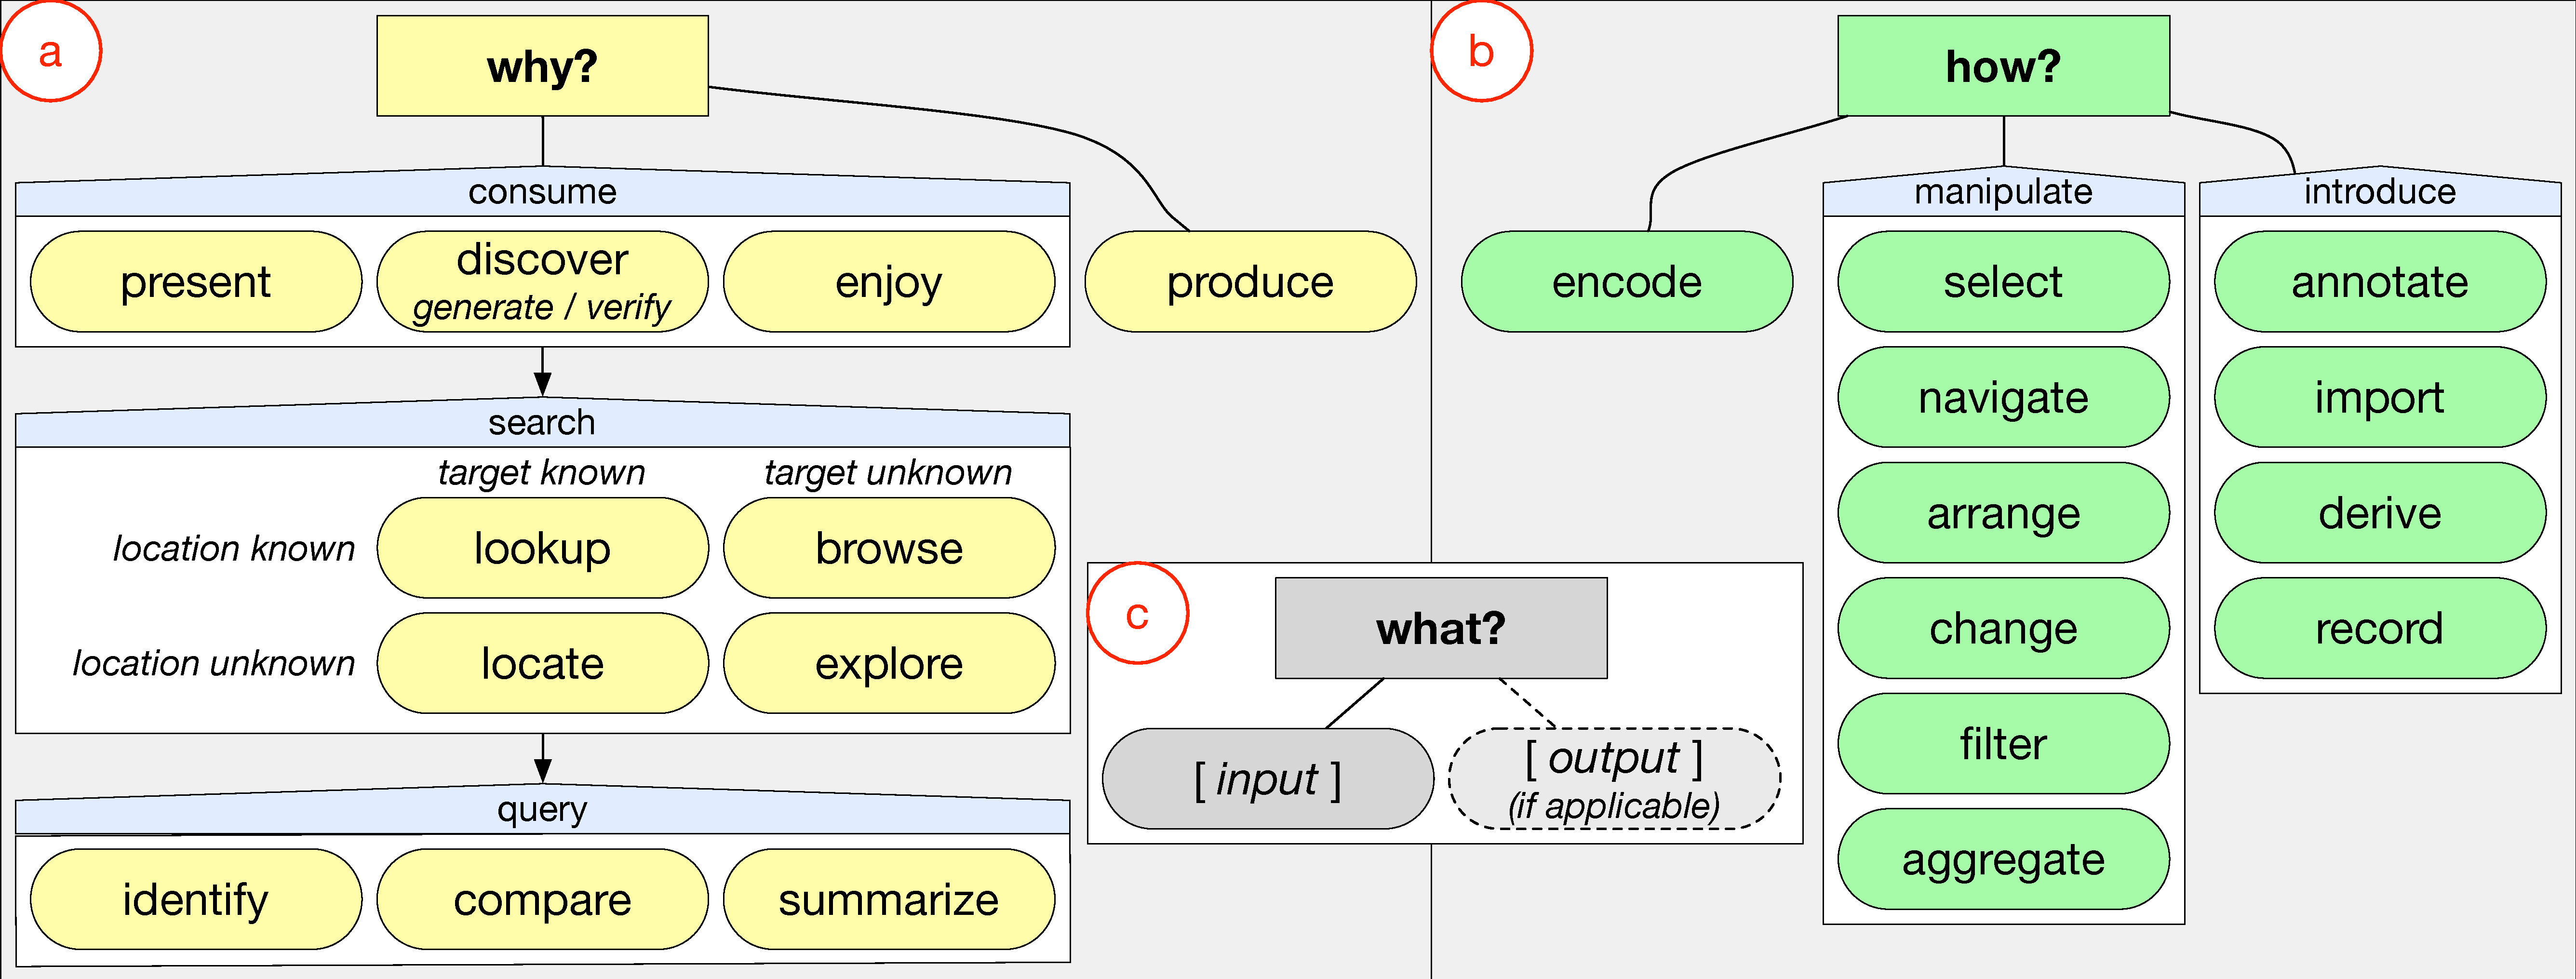
\includegraphics[width=\textwidth]{figures/typology.pdf}
    \caption
    [
        Our multi-level typology of abstract visualization tasks: \textsl{why}, \textsl{how}, and \textsl{what}.
    ]
    {
        Our multi-level typology of abstract visualization tasks.
        The typology spans \textsl{why}, \textsl{how}, and \textsl{what}; task descriptions are formed by nodes from each part:
        (a) \textsl{why} data is visualized, from high-level ({\tt consume} vs.~{\tt produce}) to mid-level ({\tt search}) to low-level ({\tt query});
        (b) \textsl{how} a visualization tool or technique supports the task in terms of visual encoding and interaction design choices;
        (c) \textsl{what} the task {\tt inputs} and {\tt outputs} are.
    }
    \label{typology:fig:typology}
\end{figure}

%-|-|-|-|-|-|-|-|-|-|-|-|-|-|-|-|-|-|-|-|-|-|-|-|-|-|-|-|-|-|-|-|-|-|-|-|-


Our multi-level typology\footnote{We denote this work as a {\it typology}, rather than a {\it taxonomy}, as the former is appropriate for classifying abstract concepts, while the latter is appropriate for classifying empirically observable events~\cite{Bailey1994}. For instance, one could construct a taxonomy of the observable ways in which a person could interact with a particular visualization tool, or a taxonomy of existing visual encoding\index{visual encoding} design choices for tree-based data~\cite{Schulz2011}.}\index{task!task typology} of abstract visualization tasks\index{task!task abstraction}, represented in \autoref{typology:fig:typology}, is encapsulated by three questions: {\it why}\index{{\tt why}} the data is being visualized, {\it how}\index{{\tt how}} the visualization tool or technique supports the task\index{task}, and {\it what}\index{{\tt what}} does the task\index{task} pertain to (\autoref{typology:fig:typology}a-c).
Complete task\index{task} descriptions, such as those for Examples \#1-2 (represented in \autoref{typology:fig:task_examples}), must include nodes from all three parts of this typology.
%RR: p.24 "taxonomy" vs "typology". The latter is apparently used for abstract concepts. But wouldn't the higher levels of a taxonomy also be abstract? If so, this distinction would apply just to the leaf nodes. And a set of existing systems would presumably be handled by a "taxonomy", but would then be discussed with reference to a "typology". Is this distinction really all that helpful? Or does it cause more confusion than it's worth?
In the remainder of this dissertation, we use a {\tt fixed-width font} to highlight vocabulary from this typology\index{task!task typology}; this vocabulary is also indexed separately at the end of this dissertation.

This structure, while unusual relative to many existing classifications, mirrors the analytical thinking process undertaken in design studies~\cite{Sedlmair2012}.
{\it Why}\index{{\tt why}}, {\it what}\index{{\tt what}}, and {\it how}\index{{\tt how}} are also used in {\it Cognitive Work Analysis} by \citet{Vicente1999}\index{cognitive work analysis (Vicente)}, particularly for relating abstractions within a work domain\index{work domain analysis}, as well as in an analysis of techniques and tools for visualizing time-oriented data by \citet{Aigner2011}, which asks {\it what is presented?}, {\it why is it presented?}, and {\it how is it presented?}.

We will introduce {\it why}\index{{\tt why}} before {\it how}\index{{\tt how}}, as this order reflects the translation of empirically observable domain problems into abstract tasks\index{task!task abstraction} and subsequently into visual encoding\index{visual encoding} and interaction\index{interaction} design choices: practitioners first determine {\it why}\index{{\tt why}} data is visualized, and then must decide upon {\it how}\index{{\tt how}} the visualization tool or technique will support the task\index{task}.
We then discuss the {\it what}\index{{\tt what}} part of our typology\index{task!task typology}, which considers the {\tt input}\index{{\tt input}} and {\tt output}\index{{\tt output}} of tasks\index{task}.
Our typology\index{task!task typology} supports the description of a complex domain-specific visualization workflow\index{workflows} as a sequence of interdependent tasks\index{task!task sequence}, where the {\tt output}\index{{\tt output}} of a prior task\index{task} may serve as the {\tt input}\index{{\tt input}} to a subsequent task\index{task}, as we demonstrate in the example featured in \autoref{typology:results}.

For clarity, we first present our typology\index{task!task typology} in its entirety with minimal discussion of the previous work that informed its organization, and then focus on these connections in \autoref{typology:rw} and in \autoref{typology:tab:rw:why} and \autoref{typology:tab:rw:how}.

%-------------------------------------------------------------------------

\subsection{Why is Data Being Visualized?}
\label{typology:why}

%-------------------------------------------------------------------------

The {\it why}\index{{\tt why}} part of our typology\index{task!task typology}, shown in \autoref{typology:fig:typology}a, allows us to describe {\it why}\index{{\tt why}} the data is being visualized, and includes multiple levels of abstraction, a narrowing of scope from high-level\index{task!high-level tasks} ({\tt consume} vs. {\tt produce}\index{{\tt produce}}) to mid-level\index{task!mid-level tasks} ({\tt search}\index{{\tt search}}) to low-level\index{task!low-level tasks} ({\tt query}\index{{\tt query}}).

\bstart{Consume}
People visualize data in order to {\tt consume}\index{{\tt consume}} information in many domain contexts.
In most cases, this consumption is driven either by a need to present information or to discover\index{{\tt discover}} and analyze new information~\cite{vanWijk2006}.
However, there are many other contexts in which the information being visualized is simply enjoyed~\cite{Dork2012,Pousman2007,Sprague2012}\index{{\tt enjoy}}, where people indulge their casual interests in a topic.

{\tt Present}\index{{\tt present}}
refers to the visualization of data for the succinct communication of information, for telling a story with data\index{storytelling}, guiding an audience through a series of cognitive operations.
Presentation using a visualization technique or tool may take place within the context of decision making, planning, forecasting, and instructional processes~\cite{Friel2001,Marchionini2006,Roth2012,Roth2013}.
Presentation brings to mind collaborative and pedagogical contexts, and the way in which a presentation is given may vary according to the size of the audience, whether the presentation is live or pre-recorded, and whether the audience is co-located with the presenter~\cite{Kosara2013}.

{\tt Discover}\index{{\tt discover}}
is about the generation and verification of hypotheses and is associated with modes of scientific inquiry~\cite{Pike2009}.
Scientific investigation may be motivated by existing theories, models, and hypotheses, or by the serendipitous observation of unexpected phenomena~\cite{Andre2009}.

{\tt Enjoy}\index{{\tt enjoy}}
refers to casual encounters with visualized data~\cite{Pousman2007,Sprague2012}.
In these contexts, a person is not driven by a need to verify\index{{\tt discover}} or generate\index{{\tt discover}} a hypothesis; novelty stimulates curiosity and thereby exploration~\cite{Dork2011,Sprague2012,Stephenson1967,Toms2000}\index{{\tt explore}}.
This motivation is notably absent from existing classifications, as shown in \autoref{typology:tab:rw:why} and \autoref{typology:tab:rw:how}.
Casual encounters with visualized data can be fleeting, such as in the earlier example of encountering a static choropleth electoral map\index{visual encoding!map!choropleth map} while reading a blog post.
Conversely, these encounters might be immersive and time-consuming experiences, such as in museum settings~\cite{Pousman2007}.

\bstart{Produce}
we use {\tt produce}\index{{\tt produce}} in reference to tasks\index{task} in which the intent is to generate new information.
This information includes but is not limited to: transformed or derived data\index{{\tt derive}}, annotations, recorded interactions\index{{\tt record}}, or screenshots of static visualizations.
Examples of {\tt produce}\index{{\tt produce}} in previous work include the production of graphical annotations and explanatory notes to describe features of line graphs\index{visual encoding!line graph} of time series data\index{time-oriented data}~\cite{Willett2012}, or the production of {\it graphical histories} in Tableau intended to document the analytical provenance\index{analytical provenance} of a person using this tool~\cite{Heer2008}.
Additional examples of {\tt produce}\index{{\tt produce}} involving derived data and annotations\index{{\tt annotate}} are featured in the example of \autoref{typology:results}.

It is important to note that the products of a {\tt produce}\index{{\tt produce}} task\index{task} may be used in some subsequent task\index{task} that may or may not involve a visualization tool or technique.
For example, some visualization tools for analyzing high-dimensional data allow people to {\tt produce}\index{{\tt produce}} new categorical attributes for labelling clustered data points in a dimensionally reduced\index{dimensionality reduction (DR)} coordinate space; these attributes might be used later for constructing a predictive model.

\bstart{Search}
Regardless of whether the intent is to {\tt present}\index{{\tt present}}, {\tt discover}\index{{\tt discover}}, or merely {\tt enjoy}\index{{\tt enjoy}}, a person will {\tt search}\index{{\tt search}} for aspects of interest in the visualized data.
While terms relating to {\tt search}\index{{\tt search}} and exploration\index{{\tt explore}} are often conflated~\cite{Marchionini2006,Toms2000}, we have imposed a characterization of {\tt search}\index{{\tt search}} that depends on {\it what}\index{{\tt what}} is being sought.
We classify them according to whether the identity or location of the search target is known a priori.
Whether the identity of the search target is known recalls the concept of {\it references} and {\it characteristics} introduced by \citet{Andrienko2006}: {\tt searching}\index{{\tt search}} for known reference targets entails {\tt lookup}\index{{\tt lookup}} or {\tt locate}\index{{\tt locate}}, while {\tt searching}\index{{\tt search}} for targets matching particular characteristics entails {\tt browse}\index{{\tt browse}} or {\tt explore}\index{{\tt explore}}.
Consider our earlier example of a person who is familiar with American geography and is {\tt searching}\index{{\tt search}} for California on an choropleth map\index{visual encoding!map!choropleth map}; we would describe this as an instance of {\tt lookup}\index{{\tt lookup}}.
However, a person who is {\it unfamiliar} with American geography must {\tt locate}\index{{\tt locate}} California.

In contrast, the identity of a search target might be unknown a priori; a person may be {\tt searching}\index{{\tt search}} for characteristics rather than references~\cite{Andrienko2006}; these characteristics might include particular values, extremum, anomalies, trends, or  ranges~\cite{Amar2005}.
For instance, if a person using a tree-based visual encoding\index{visual encoding!tree} is {\tt searching}\index{{\tt search}} within a particular subtree for leaf nodes having few siblings, we would describe this as an instance of {\tt browse}\index{{\tt browse}} because the location is known a priori.
Finally, {\tt explore}\index{{\tt explore}} entails {\tt searching}\index{{\tt search}} for characteristics without regard to their location; many visualization tools provide an overview of the data, which is often the starting point for exploration\index{{\tt explore}}.
Examples include {\tt searching}\index{{\tt search}} for outliers in a scatterplot\index{visual encoding!scatterplot}, for anomalous spikes or periodic patterns in a line graph\index{visual encoding!line graph} of time series data\index{time-oriented data}, or for unanticipated spatially-dependent patterns in a choropleth map\index{visual encoding!map!choropleth map}.

\bstart{Query}\index{{\tt query}}
Once a target or set of targets has been found, a person will
{\tt identify}\index{{\tt identify}}, {\tt compare}\index{{\tt compare}}, or {\tt summarize}\index{{\tt summarize}} these targets.
If a search returns known or {\it reference} targets~\cite{Andrienko2006}, either by {\tt lookup}\index{{\tt lookup}} or {\tt locate}\index{{\tt locate}}, {\tt identify}\index{{\tt identify}} returns their {\it characteristics}.
For example, someone who uses a choropleth map\index{visual encoding!map!choropleth map} representing election results can {\tt identify}\index{{\tt identify}} the winning candidate and margin of victory for the state of California.
Conversely, if a search returns targets matching particular {\it characteristics}, either by {\tt browse}\index{{\tt browse}} or {\tt explore}\index{{\tt explore}}, {\tt identify}\index{{\tt identify}} returns {\it references}.
For instance, our election map\index{visual encoding!map!choropleth map} enthusiast can {\tt identify}\index{{\tt identify}} the state having the highest margin of victory.

The progression from {\tt identify}\index{{\tt identify}} to {\tt compare}\index{{\tt compare}} to {\tt summarize}\index{{\tt summarize}} corresponds to an increase in the amount of search targets under consideration~\cite{Andrienko2006,Buja1996,Tweedie1997}, in that {\tt identify}\index{{\tt identify}} refers to a single target, {\tt compare}\index{{\tt compare}} refers to multiple subsets of targets, and {\tt summarize}\index{{\tt summarize}} refers to a whole set of targets.
As with {\tt explore}\index{{\tt explore}}, {\tt summarize}\index{{\tt summarize}} is also often associated with overviews of the data~\cite{Lee2006}.
Continuing with the choropleth map\index{visual encoding!map!choropleth map} example, the person {\tt identifies}\index{{\tt identify}} the election results for one state, {\tt compares}\index{{\tt compare}} the election results of one state to another, or {\tt summarizes}\index{{\tt summarize}} the election results across all states, determining how many favoured one candidate or the other, or the overall distribution of margin of victory values.

%-------------------------------------------------------------------------

\subsection{How Does the Visualization Technique or Tool Support the Task?}
\label{typology:how}

%-------------------------------------------------------------------------


We now turn our consideration to the {\it how}\index{{\tt how}} part of our typology\index{task!task typology}, which contains {\it idioms}, defined as families of related visual encoding\index{visual encoding} and interaction\index{interaction} design choices.
This part of our typology\index{task!task typology}, shown in \autoref{typology:fig:typology}b, is likely to be most familiar to readers, as it contains a number of {\it idioms} associated with interaction\index{interaction} design choices that are well-represented by several existing classifications \cite{Gotz2008,Mullins1993,Roth2012,Roth2013,Yi2007}.
%RR: p, 28 - Are idioms essentially alternate ways of carrying out a process? If so, perhaps compare them with the design templates sometimes proposed for architecture. (Alexander - a pattern language)
We distinguish between three classes of idioms: those for {\tt encoding}\index{{\tt encode}} data, those for {\tt manipulating}\index{{\tt manipulate}} previously encoded elements, and those for {\tt introducing} new elements.

\bstart{Encode}
The majority of visualization tasks\index{task} rely on {\it how}\index{{\tt how}} data is initially encoded\index{{\tt encode}} as a visual representation\footnote{Some tasks do not depend on {\it how} the data is visually encoded, or take place before the data is encoded; consider, for instance, {\tt produce} tasks that involve {\tt deriving} new data or {\tt recording} states of a visual analysis process or presentation for downstream consumption.}.
A full enumeration of visual encoding\index{visual encoding} design choices for various datatypes beyond the scope of this chapter and appears in Munzner's book~\cite{Munzner2014}.

\bstart{Manipulate}\index{{\tt manipulate}} 
The following idioms affect previously encoded\index{{\tt encode}} elements, modifying them to some extent.
These idioms represent families of interrelated design choices incorporating both interaction\index{interaction} and visual encoding\index{visual encoding}.
We consider visual encoding\index{visual encoding} and interaction\index{interaction} design choices in a unified way because many idioms incorporate aspects of both~\cite{Meyer2015,Munzner2009}, such as focus + context\index{view coordination!focus + context} techniques~\cite{Grosjean2002,Munzner2003}.

{\tt Select}\index{{\tt select}}
refers to the demarcation of one or more encoded\index{{\tt encode}} elements, differentiating selected from unselected elements~\cite{Raskin2000}.
Examples range from directly clicking or lassoing elements in a scatterplot\index{visual encoding!scatterplot} to brushing\index{view coordination!brushing across views} design choices used to highlight elements in visualization tools incorporating multiple linked views~\cite{Weaver2007}\index{view coordination}.

{\tt Navigate}\index{{\tt navigate}}
refers to instances where the person using a visualization tool or technique alters their viewpoint, such as zooming, panning, and rotating.
Other navigation instances include the triggering of details-on-demand\index{view coordination!details-on-demand} views, combining {\tt navigate}\index{{\tt navigate}} and {\tt select}\index{{\tt select}}~\cite{Shneiderman1996}.

{\tt Arrange}\index{{\tt arrange}}
refers to the process of organizing encoded\index{{\tt encode}} elements spatially.
This includes arranging representations of data~\cite{Liu2010,Mullins1993,Wilkinson2005}, such as reordering the axes in a parallel coordinates plot\index{visual encoding!parallel coordinates plot} or the rows and columns of a \ac{SPLOM}\index{visual encoding!scatterplot!scatterplot matrix (SPLOM)}.
Other forms of arrangement allow people to coordinate the spatial layout of views~\cite{Heer2012,Weaver2007}\index{view coordination}.

{\tt Change}\index{{\tt change}}
pertains to alterations in visual encoding\index{visual encoding}.
Simple examples include altering the size and transparency of points in a scatterplot\index{visual encoding!scatterplot} or edges in a node-link graph\index{visual encoding!node-link graph}, altering a colour-scale or texture mapping, or transforming the scales of axes.
Other alterations have more pronounced effects, changing the visual encoding\index{visual encoding}, such as transitioning between grouped\index{visual encoding!bar chart!grouped bar chart} and stacked bar charts\index{visual encoding!bar chart!stacked bar chart}, or between linear and radial layouts for line graphs\index{visual encoding!line graph} of time series data\index{time-oriented data}.
Pronounced changes in visual encoding\index{visual encoding} such as these are often facilitated by smoothly animated transitions\index{view coordination!animated transitions}, which reduce their disruptive effects~\cite{Heer2007}.

{\tt Filter}\index{{\tt filter}}
refers to adjustments to the exclusion and inclusion criteria for encoded\index{{\tt encode}} elements.
Some forms of filtering allow for elements to be temporarily hidden from view and later restored, while other forms are synonymous with outright deletion.
As an example of temporary {\tt filtering}\index{{\tt filter}}, consider a person examining an age histogram\index{visual encoding!histogram} based on population census data.
First, she decides to exclude males, then further adjusts her filter criteria to focus solely on unemployed females.
Finally, she revises the gender criteria to focus on unemployed males.

A common example of permanent {\tt filtering}\index{{\tt filter}}, or deletion, is that of manually {\tt selecting}\index{{\tt select}} and removing outliers resulting from errors in data entry.
Alternatively, consider a scatterplot\index{visual encoding!scatterplot} in which some data points are labelled with manually generated categorical tags.
Deleting a tag would remove this categorical label from all data points having that tag.

{\tt Aggregate}\index{{\tt aggregate}}
concerns changes in the granularity of encoded\index{{\tt encode}} elements; we also consider its converse, segregate, as being associated with this family of design choices.
For example, a person may adjust the granularity of a continuous time scale in a line graph\index{visual encoding!line graph}, aggregating daily values into monthly values, or segregating annual values into quarterly values.
Alternatively, a person may aggregate a clique within a node-link graph\index{visual encoding!node-link graph} into a representative glyph, or segregate clique glyphs into their component nodes.

\bstart{Introduce}
While {\tt manipulate}\index{{\tt manipulate}} idioms alter previously encoded\index{{\tt encode}} elements, {\tt introduce} idioms add new elements.

{\tt Annotate}\index{{\tt annotate}}
refers to the addition of graphical or textual annotations associated with one or more encoded\index{{\tt encode}} elements.
When an annotation is associated with data elements, an annotation could be thought of as a new attribute for these elements.
The earlier example of manually tagging points in a scatterplot\index{visual encoding!scatterplot} with categorical labels is one such instance of annotating data.

{\tt Import}\index{{\tt import}}
pertains to the addition of new data elements.
In some environments, these new data elements might be loaded from external sources, while others might be manually generated.

{\tt Derive}\index{{\tt derive}}
refers to the computation of new data elements given existing data elements.
Aggregating\index{{\tt aggregate}} data often implies deriving data, however this may not always be true: we further specify that derived data must be persistent, while aggregated data need not be.
For instance, a person might {\tt derive} new attributes for tabular data using a \ac{MDS}\index{dimensionality reduction (DR)!multi-dimensional scaling (MDS)} algorithm.

Finally, {\tt record}\index{{\tt record}}
refers to the saving or capturing of elements as persistent artefacts.
As a consequence, {\tt record}\index{{\tt record}} is often associated with {\tt produce}\index{{\tt produce}}.
These artefacts include screen shots, annotations, lists of bookmarked elements or locations, parameter settings, or interaction logs~\cite{Shrinivasan2008}\index{interaction!interaction logs}.
An interesting example of {\tt record}\index{{\tt record}} is that of assembling a {\it graphical history}~\cite{Heer2008}, in which the {\tt output}\index{{\tt output}} of each task\index{task} includes a static snapshot of the state of the visualization tool, and as these snapshots accumulate they are encoded\index{{\tt encode}} as a branching tree\index{visual encoding!tree}.
{\tt Recording}\index{{\tt record}} and retaining artefacts such as these are often desirable for maintaining a sense of analytical provenance\index{analytical provenance}, allowing people who use the tool to revisit earlier states or parameter settings.

%-------------------------------------------------------------------------

\subsection{What are the Inputs and Outputs of the Task?}
\label{typology:what}

%-------------------------------------------------------------------------

Previous work has reached no agreement on the question of {\it what}\index{{\tt what}} is visualized.
Many classifications do not address it at all; others discuss {\it what}\index{{\tt what}} implicitly, as indicated by the parenthetical terms in \autoref{typology:tab:rw:why} and \autoref{typology:tab:rw:how}.
Of those that classify {\it what}\index{{\tt what}}, some focus on the level of the entire dataset, such as {\it tables} composed of {\it values} and {\it attributes} or {\it networks} composed of {\it nodes} and {\it links}~\cite{Shneiderman1996}.
Others allow more precise specification of data-attribute semantics, such as {\it categorical}, {\it ordinal}, and {\it quantitative}~\cite{Card1999}.
A few classifications include not only {\it data} but also {\it views} as first-class citizens~\cite{Chi1998,Chuah1996,Heer2012,Ward2004}\index{view coordination}.
Specific examples of {\it what}\index{{\tt what}} as classified in previous work include: 

\begin{itemize}

    \item Values, extremum, ranges, distributions, anomalies, clusters, correlations~\cite{Amar2005}.
    
    \item {\it Graph-specific objects}~\cite{Lee2006}: nodes, links, paths, graphs, connected components, clusters, groups.
    
    \item {\it Time-oriented primitives}~\cite{Aigner2011}: points, intervals, spans, temporal patterns, rates of change, sequences, synchronization.
    
    \item {\it Interaction operands}~\cite{Ward2004}: pixels, data [values, structures], attributes, geometric [objects, surfaces], visualization structures.
    
\end{itemize}

%-|-|-|-|-|-|-|-|-|-|-|-|-|-|-|-|-|-|-|-|-|-|-|-|-|-|-|-|-|-|-|-|-|-|-|-|-

In this typology\index{task!task typology}, we have chosen a flexible and agnostic representation of {\it what}\index{{\tt what}} that accommodates all of these modes of thinking: in short, we have a ``bring your own {\it what}\index{{\tt what}}'' mentality.
The only absolute requirement is to explicitly distinguish a task's\index{task} {\tt input}\index{{\tt input}} and {\tt output}\index{{\tt output}} constraints when describing sequences of interdependent tasks~\cite{Tweedie1997}\index{task!task sequence}.
An extensive discussion of {\it what}\index{{\tt what}} that dovetails well with this typology\index{task!task typology} appears in Munzner's book~\cite{Munzner2014}\footnote{\citet{Munzner2014} provides a structured classification of data as well as a classification of {\it targets}; both can be used in the analysis of {\tt inputs} and {\tt outputs}. 
The classification of {\it targets} is represented in \autoref{fig:typology-targets}.}. %, but it cannot be effectively summarized in a few paragraphs; thus, it is beyond the scope of this chapter.
% RR: p. 32. - "[what] cannot be effectively summarized in a few paragraphs." Really? This is a very Wittgensteinian remark. What makes you believe that it cannot be summarized? Things that cannot be compressed are usually regarded as random noise. Is there no central point?


%-------------------------------------------------------------------------

\subsection{Concise Task Descriptions}
\label{typology:task descriptions}

%-------------------------------------------------------------------------

Our multi-level typology\index{task!task typology} can be used to concisely describe visualization tasks\index{task}.
Each task\index{task} is defined by {\it why}\index{{\tt why}} data is being visualized, {\it how}\index{{\tt how}} the visualization tool or technique supports the task\index{task}, and by {\it what}\index{{\tt what}} are the {\tt inputs}\index{{\tt input}} and {\tt outputs}\index{{\tt output}} of the task\index{task}.
Single tasks\index{task} may involve multiple nodes from each part of the typology\index{task!task typology}, as shown in \autoref{typology:fig:task_examples}.

%-|-|-|-|-|-|-|-|-|-|-|-|-|-|-|-|-|-|-|-|-|-|-|-|-|-|-|-|-|-|-|-|-|-|-|-|-

\begin{figure}
    \centering
    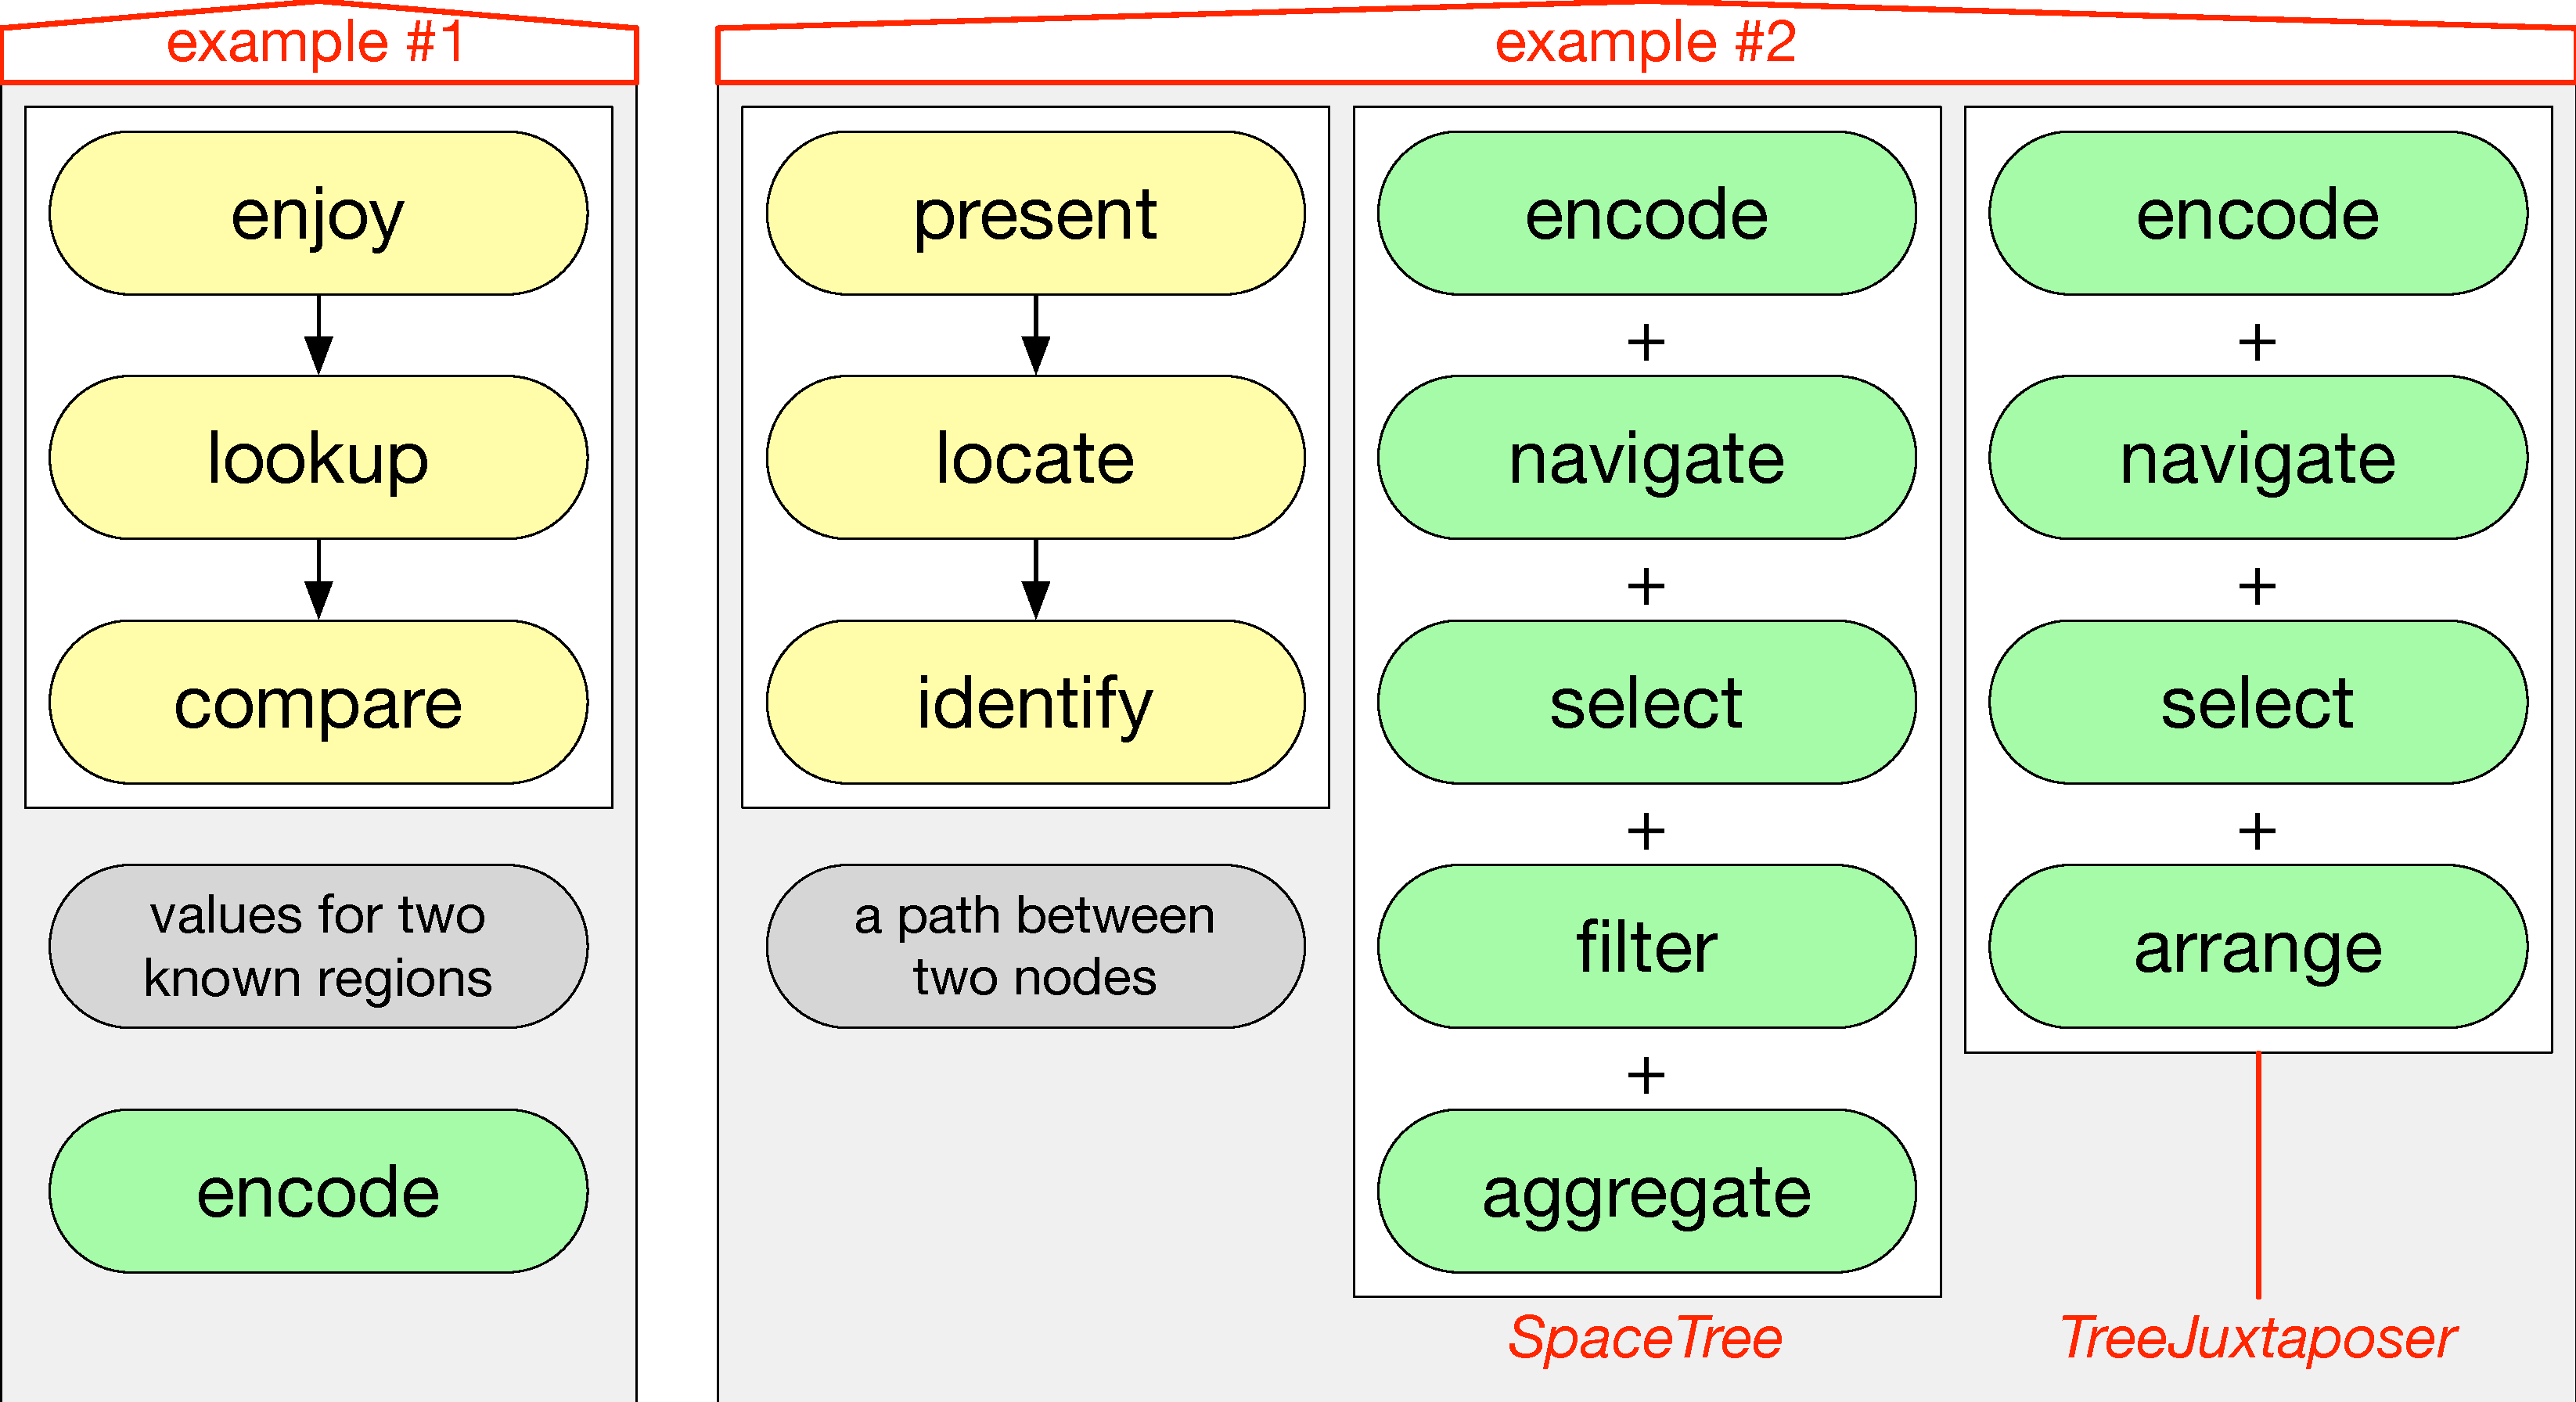
\includegraphics[width=\textwidth]{figures/task_examples.pdf}
    \caption
    [
        Task descriptions for Example \#1 (choropleth map) and Example \#2 (large trees).
    ]
    {
        Task descriptions for Example \#1 (left): casually encountering an choropleth electoral map and comparing election results for two regions; and Example \#2 (right): presenting a path between two nodes in a large tree using SpaceTree~\cite{Grosjean2002} and TreeJuxtaposer~\cite{Munzner2003}.
    }
    \label{typology:fig:task_examples}
\end{figure}

%-|-|-|-|-|-|-|-|-|-|-|-|-|-|-|-|-|-|-|-|-|-|-|-|-|-|-|-|-|-|-|-|-|-|-|-|-

We have chosen to present these descriptions using a simple and flexible visual notation, rather than with a formal grammar~\cite{Andrienko2006,Lammarsch2012,Schulz2013,Tweedie1997,Wilkinson2005}; in doing so, creating and iterating on task\index{task} descriptions can be easily integrated into existing collaborative design and ideation activities, making use of materials such as coloured sticky notes and whiteboards.
A crucial aspect of these descriptions is that sequences of interdependent tasks\index{task} can be chained together\index{task!task sequence}, such that the {\tt output}\index{{\tt output}} from earlier tasks\index{task} forms the {\tt input}\index{{\tt input}} to later tasks\index{task}, as discussed in the following example and as represented in \autoref{typology:fig:task_chain}.

%-------------------------------------------------------------------------
%-------------------------------------------------------------------------

\section{Example: A Sequence of Interdependent Tasks}
\label{typology:results}

%-------------------------------------------------------------------------
%-------------------------------------------------------------------------

%-|-|-|-|-|-|-|-|-|-|-|-|-|-|-|-|-|-|-|-|-|-|-|-|-|-|-|-|-|-|-|-|-|-|-|-|-

\begin{figure}
    \centering
    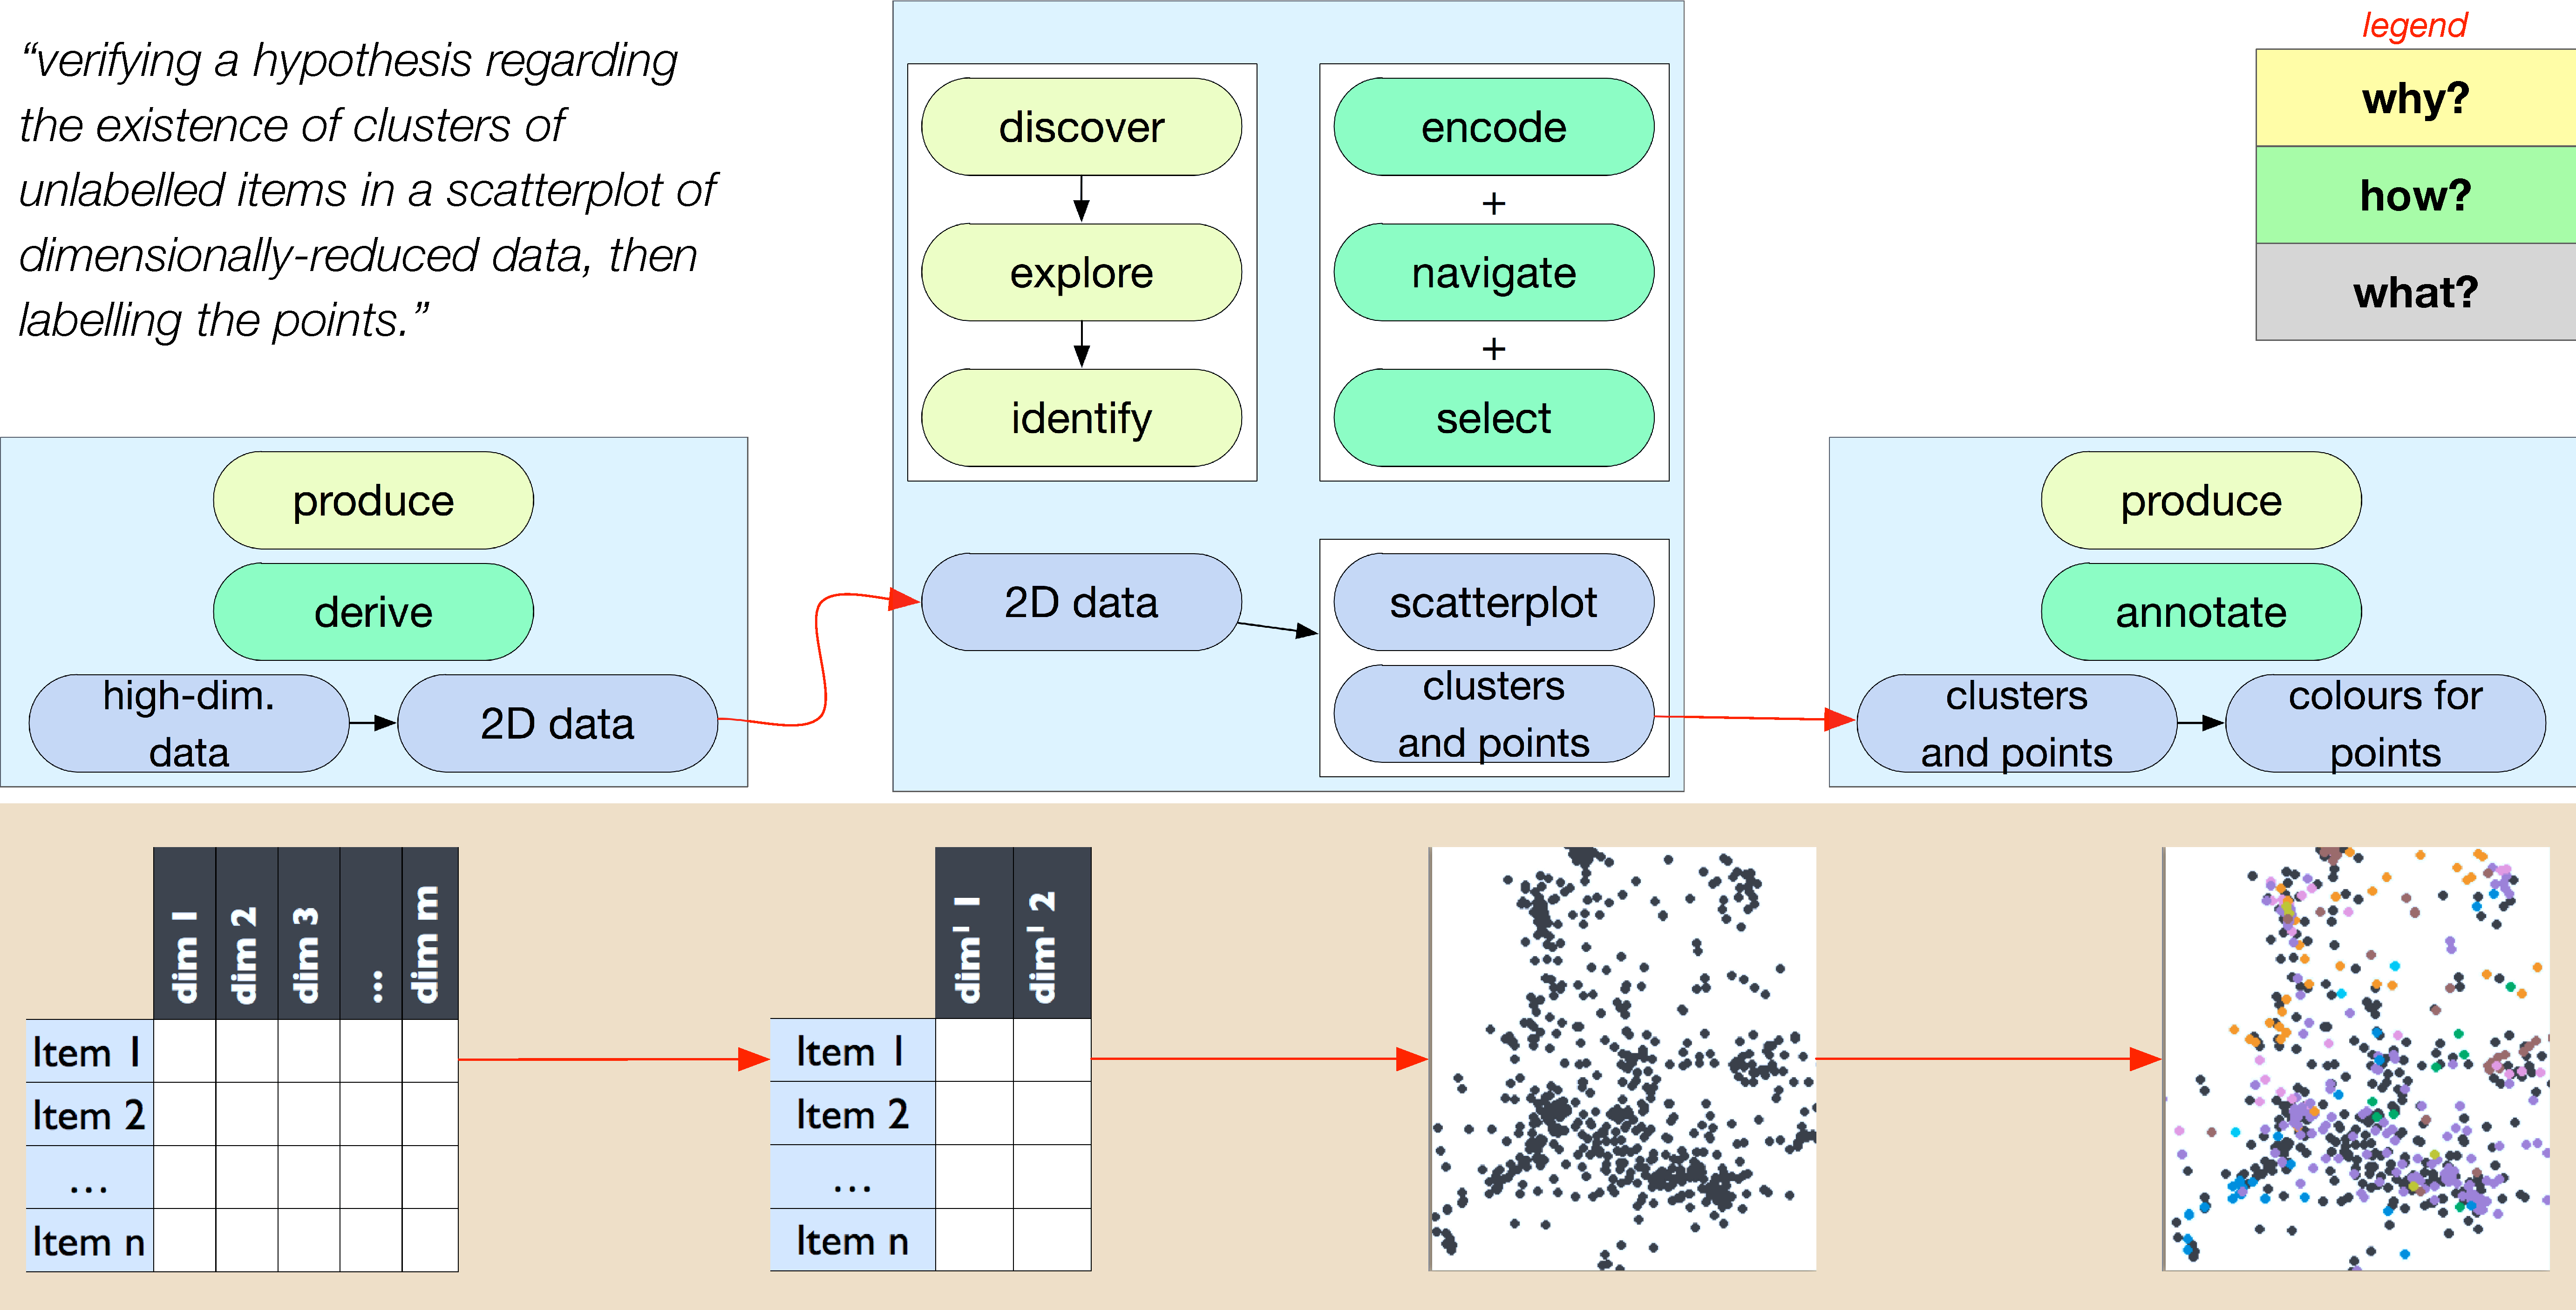
\includegraphics[width=\textwidth]{figures/typology-example.pdf}
    \caption
    [
        An example sequence of tasks as using the structure and vocabulary of our typology.
    ]
    {
        An example sequence of tasks, described as a sentence (top left), as well as using the structure and vocabulary of our typology (top); the bottom depicts a series of transformations corresponding to the {\tt inputs} and {\tt outputs} of each task.
    }
    \label{typology:fig:task_chain}
\end{figure}

%-|-|-|-|-|-|-|-|-|-|-|-|-|-|-|-|-|-|-|-|-|-|-|-|-|-|-|-|-|-|-|-|-|-|-|-|-

Visualization tasks\index{task} are seldom executed in isolation, and the {\tt output}\index{{\tt output}} of one task\index{task} may serve as {\tt input}\index{{\tt input}} to a subsequent task\index{task!task sequence}.
To illustrate this type of dependency, we present an example in which our typology\index{task!task typology} is used to describe a sequence of interdependent tasks\index{task!task sequence}.

Consider the case of labelling clusters of related items in a dataset with many dimensions, where a label is a new categorical attribute value for the item.
Labels are assigned to clusters by means\index{task!means} of {\tt annotation}\index{{\tt annotate}}.
However, one must first {\tt explore}\index{{\tt explore}} the visualized dataset and {\tt identify}\index{{\tt identify}} clusters of interest.
Here a person uses a visualization technique in which items in the dataset are {\tt encoded}\index{{\tt encode}} as points in an interactive scatterplot\index{visual encoding!scatterplot}.
{\tt Identifying}\index{{\tt identify}} clusters is facilitated by {\tt navigating}\index{{\tt navigate}} and {\tt selecting}\index{{\tt select}} items in this scatterplot\index{visual encoding!scatterplot}; upon {\tt selection}\index{{\tt select}}, additional attribute values for the item are shown in details-on-demand\index{view coordination!details-on-demand} secondary displays or in tooltips.
This task\index{task} too has a dependency on the result of an earlier task\index{task}.
Before the the data is {\tt encoded}\index{{\tt encode}} in the scatterplot\index{visual encoding!scatterplot}, a set of two-dimensional distances between data points must be {\tt produced}\index{{\tt produce}}:     they are {\tt derived}\index{{\tt derive}} from the original set of dimensional attributes using \ac{DR}\index{dimensionality reduction (DR)}.

Using our typology\index{task!task typology}, we can express dependencies in which the {\tt output}\index{{\tt output}} of one task\index{task} serves as the {\tt input}\index{{\tt input}} of another, such as the relationship between how data is {\tt derived}\index{{\tt derive}} and the choice of visual encoding\index{visual encoding}.
Such dependencies are represented in \autoref{typology:fig:task_chain}.

As in the examples of \autoref{typology:context}, we can compare our description to those generated by other classifications.
Consider the classification of basic visualization tasks\index{task} by \citet{Chuah1996}, which distinguishes between three categories of {\it operations}.
Using this classification, this sequence of tasks\index{task!task sequence} could be described as having {\it data operations} ({\it derived attributes}\index{{\tt derive}}), {\it graphical operations} ({\it encode data}\index{{\tt encode}}), and {\it set operations} ({\it create set, express membership}).
This description does specify {\it how}\index{{\tt how}} and {\it what}\index{{\tt what}}, but it does not express the interdependencies within a sequence of tasks\index{task!task sequence}, nor does it tell us {\it why}\index{{\tt why}} the data is being visualized.
Neither can we easily distinguish when sets (or clusters) are created, as this might occur before the data is encoded\index{{\tt encode}}, or it might occur via interactive {\tt selection}\index{{\tt select}} of items in the scatterplot\index{visual encoding!scatterplot}.

While the description based on \citet{Chuah1996} classification is atemporal, the {\it operator} {\it interaction} {\it framework} by \citet{Chi1998} defines stage- and transformation- based operators occurring along the visualization pipeline.
Their framework does not contain a comprehensive list of operators, so we draw from the example {\it operators} cited in their paper to describe this sequence of tasks\index{task!task sequence} as follows:

%-|-|-|-|-|-|-|-|-|-|-|-|-|-|-|-|-|-|-|-|-|-|-|-|-|-|-|-|-|-|-|-|-|-|-|-|-

\begin{enumerate}
    \item {\it visualization transformation operators}: \\
    dimension reduction (\ac{DR})\index{dimensionality reduction (DR)}
    
    \item {\it visual mapping transformation operators}: \\
    scatterplot\index{visual encoding!scatterplot}
    
    \item {\it view stage operators}: \\
    zoom, focus, details-on-demand\index{view coordination!details-on-demand}, pick

\end{enumerate}

%-|-|-|-|-|-|-|-|-|-|-|-|-|-|-|-|-|-|-|-|-|-|-|-|-|-|-|-|-|-|-|-|-|-|-|-|-

This description does capture the interdependencies for this sequence of tasks\index{task!task sequence}, though it mischaracterizes the processes of dimension reduction\index{dimensionality reduction (DR)} as transformations to visualized elements, rather than transformations on data, a distinction central to our definition of {\tt derive}\index{{\tt derive}}.
While this description captures up until the second task\index{task} in our description, it does not capture the final task\index{task} of producing cluster labels by means\index{task!means} of annotation\index{{\tt annotate}}.

The description based on our typology retains the separability of these tasks\index{task}, ensuring the distinction between interim {\tt inputs}\index{{\tt input}} and {\tt outputs}\index{{\tt output}}.
Another problem with descriptions generated by existing classifications was that of coverage; the {\it how}\index{{\tt how}} part of our typology includes both {\tt derive}\index{{\tt derive}} and {\tt annotate}\index{{\tt annotate}}, while descriptions generated by other classifications could not account for the latter~\cite{Amar2005,Chi1998}, or both~\cite{Pike2009,Shneiderman1996,Valiati2006,Wehrend1990,Yi2007,Zhou1998}.
Finally, our description also accounts for both {\it why}\index{{\tt why}} data is {\tt derived}\index{{\tt derive}} and {\it why}\index{{\tt why}} clusters are {\tt annotated}\index{{\tt annotate}} with tags, whereas descriptions generated using existing classifications mention {\it how}\index{{\tt how}} a task\index{task} is performed in relation only to {\it when} it is performed~\cite{Chi1998} or to {\it what}\index{{\tt what}} it is performed on~\cite{Chuah1996}.
We maintain that a task\index{task} description requires {\it why}\index{{\tt why}}, {\it how}\index{{\tt how}}, and {\it what}\index{{\tt what}}; the question of {\it when} for a sequence of interdependent tasks\index{task!task sequence} is best served by denoting task\index{task} {\tt input}\index{{\tt input}} and {\tt output}\index{{\tt output}}.

%-------------------------------------------------------------------------
%-------------------------------------------------------------------------

\section{Connections to Previous Work}
\label{typology:rw}

%-------------------------------------------------------------------------
%-------------------------------------------------------------------------

Our typology was informed in part by related work, including existing classifications and established theoretical models, and in part by new thinking with many points of divergence from previous work.
We surveyed work relating to tasks\index{task} spanning the research literature in visualization, visual analytics\index{visual analytics}, \ac{HCI}\index{human-computer interaction (HCI)}, cartography\index{cartography}, and information retrieval\index{information retrieval}.
We focus on two subsets that informed the configuration of our typology: thirty works that explicitly contribute a taxonomy, typology, characterization, framework, or model of tasks\index{task}, goals, objectives, intentions, activities, or interactions~\cite{Amar2005,Amar2004,Andrienko2006,Buja1996,Card1999,Casner1991,Chi1998,Chuah1996,Dix1998,Gotz2008,Heer2012,Keim2002,Klein2006,Lee2006,Liu2010,Mullins1993,Pike2009,Pirolli2005,Raskin2000,Roth2012,Roth2013,Roth1990,Shneiderman1996,Spence2007,Springmeyer1992,Tweedie1997,Valiati2006,Ward2004,Wehrend1990,Yi2007,Zhou1998}\index{interaction}, along with twenty other references that make compelling or noteworthy assertions about the behaviour of people who use visualization tools or techniques~\cite{Aigner2011,Andre2009,Dork2011,Dork2012,Friel2001,Kandel2012,Marchionini2006,Munzner2009a,Plaisant1995,Pousman2007,Roth2012a,Sprague2012,Shrinivasan2008,Stephenson1967,Tory2004,Toms2000,Tukey1977,vanWijk2006,Ware2012,Wilkinson2005}\footnote{\autoref{app:typology} includes additional meta-analysis of this literature and documents the evolution of our typology.}.
The similarities between the individual nodes of our typology and those of existing classifications and other related work are presented in detail in \autoref{typology:tab:rw:why} and \autoref{typology:tab:rw:how}\footnote{\citet{Yalcin2014} has visualized the vocabulary from previous work represented in these tables here: \url{http://keshif.me/demo/vis_tasks.html}.}.

\autoref{typology:tab:rw:why} and \autoref{typology:tab:rw:how} serve three purposes: they document our choices of terms for the purpose of reproducibility, they illustrate the influence of previous work on our thinking, and they indicate overrepresented and underrepresented areas in the literature, such as {\tt consume}\index{{\tt consume}} and {\tt enjoy}\index{{\tt enjoy}} in the {\it why}\index{{\tt why}} part of our typology.
Note that non-leaf nodes in the {\it how}\index{{\tt how}} part of our typology are poorly represented, serving to indicate the gap between low and high levels of abstraction\index{task!task abstraction}.

%-|-|-|-|-|-|-|-|-|-|-|-|-|-|-|-|-|-|-|-|-|-|-|-|-|-|-|-|-|-|-|-|-|-|-|-|-

\begin{table}\renewcommand{\arraystretch}{1.2}\addtolength{\tabcolsep}{-1pt}
    \begin{center}
    \tiny
    \begin{tabular}{p{0.125\textwidth}>{\RaggedRight}p{0.8\textwidth}}
    
    \rowcolor{yellow!20} 
    
        \multicolumn{2}{c}{\it why?} 
        
    \\
    
    \hline
    
    \rowcolor{blue!10}
    
        {\tt consume}\index{{\tt consume}} & --
    
    \\
    
        {\tt $\rightarrow$ present}\index{{\tt present}} &
    
        	{\it \underline{present}},~\cite{Shrinivasan2008,vanWijk2006}, %Dibiase1990,
        	{\it author, compose}~\cite{Card1999}*,
        	{\it build (case), tell (story)}~\cite{Pirolli2005}*,
        	{\it depict}~\cite{Pike2009}*,
        	{\it express (ideas), describe}~\cite{Springmeyer1992}*,
        	{\it guide, share}~\cite{Heer2012}*
        	{\it inform, elaborate}~\cite{Zhou1998}*,
        	{\it report}~\cite{Kandel2012},
    
    \\ \rowcolor{gray!10}
    
        {\tt $\rightarrow$ discover (generate\index{{\tt discover}}, verify\index{{\tt discover}} hypotheses)}\index{{\tt discover}} &
    
        	{\it \underline{discover}}~\cite{Marchionini2006}, %Dibiase1990,
        	{\it explore}~\cite{Zhou1998}*, \cite{vanWijk2006},
        	{\it verify}~\cite{Casner1991}*, \cite{Marchionini2006},
        	{\it synthesize}~\cite{Mullins1993}*, \cite{Marchionini2006}, %Dibiase1990,
        	{\it investigate, integration (of insight)}~\cite{Springmeyer1992}*, \cite{Marchionini2006},
        	{\it frame operations: construct, elaborate, question, reframe}~\cite{Klein2006}*,
        	{\it assimilate, assess, understand}~\cite{Pike2009}*,
        	{\it infer}~\cite{Valiati2006}*,
        	{\it analyze}~\cite{Mullins1993,Pike2009}*, \cite{Marchionini2006},
        	{\it support, reevaluate (hypotheses)}~\cite{Pirolli2005}*, %Dibiase1990,
        	{\it monitoring}~\cite{Ware2012},
        	{\it confirm (hypotheses)},
        	{\it expose (uncertainty)},
        	{\it formulate (cause and effect)},
        	{\it concretize (relationships)},
        	{\it learn (domain parameters)},
        	{\it multivariate explanation}~\cite{Amar2004}*,
        	{\it evaluate, learn, investigate}~\cite{Marchionini2006},
        	{\it open-ended exploration, diagnosis}~\cite{Plaisant1995},
        	{\it abduction, deduction, induction}~\cite{Pike2009},
        	{\it generate, confirm (hypotheses)}~\cite{Andre2009,Friel2001}, %Dibiase1990,
        	{\it integrate, interpret}~\cite{Friel2001},
        	{\it exploratory and confirmatory data analysis}~\cite{Tukey1977} %Dibiase1990,
    
    \\
    
        {\tt $\rightarrow$ enjoy}\index{{\tt enjoy}} &
    
    	    (using visualized data in casual contexts)~\cite{Pousman2007,Sprague2012},
    	    {\it strolling}~\cite{Dork2012}
    
    \\ \rowcolor{blue!10}
    
        {\tt produce}\index{{\tt produce}} &
    
        	{\it export}~\cite{Roth2012,Roth2013}*,
        	{\it store}~\cite{Mullins1993}*,
        	{\it save}~\cite{Liu2010,Roth2012,Roth2013}*,
        	{\it extract}~\cite{Card1999,Shneiderman1996}*,
        	{\it generating (images)}~\cite{Plaisant1995},
        	(a {\it classification})~\cite{Card1999,Springmeyer1992}*,
        	(a {\it categorization})~\cite{Mullins1993,Wehrend1990,Zhou1998}*,
        	%{\it names (for clusters)}~\cite{Sedlmair2012}*,
        	(a {\it record} of one's history / process)~\cite{Heer2012,Shneiderman1996,Springmeyer1992}*
        	
        
    
    \\  \hline \rowcolor{blue!10} 
    
        {\tt search}\index{{\tt search}} &
    
            {\it \underline{search}}~\cite{Card1999,Pirolli2005,Zhou1998}*,
            {\it acquire}~\cite{Mullins1993}*,
            {\it visual queries}~\cite{Ware2012}
    
    \\
    
        {\tt $\rightarrow$ lookup}\index{{\tt lookup}} &
    
        	{\it \underline{lookup}}~\cite{Casner1991}*~\cite{Marchionini2006},
        	{\it identify: lookup (value)}~\cite{Wehrend1990}*,
        	{\it (value) lookup}~\cite{Roth1990}*,
        	{\it retrieve (value)}~\cite{Amar2005,Lee2006,Pike2009,Roth2012,Roth2013}*\cite{Tory2004},
        	{\it procure}~\cite{Roth2012,Roth2013}*
    
    \\ \rowcolor{gray!10}
    
        {\tt $\rightarrow$ browse}\index{{\tt browse}} &
    
            {\it \underline{browse}}~\cite{Card1999,Mullins1993,Pike2009,Spence2007}*, \cite{Dork2012,Toms2000}, %Tufte1997},
        	{\it search}~\cite{Roth2012,Roth2013}*, %Roth's definition of search = browse
        	{\it finding (gestalt)}~\cite{Buja1996}*,
        	{\it browsing tasks: follow (path)}~\cite{Lee2006}*
    
    \\
    
        {\tt $\rightarrow$ locate}\index{{\tt locate}} &
    
            {\it \underline{locate}}~\cite{Liu2010,Mullins1993,Valiati2006,Wehrend1990,Zhou1998}*, \cite{Friel2001},
        	{\it search}~\cite{Casner1991}*\cite{Dork2012},
        	{\it search (for known item)}~\cite{Marchionini2006},
        	{\it seek}~\cite{Spence2007}*,
        	{\it pathfinding}~\cite{Ware2012}
    
    \\ \rowcolor{gray!10}
    
        {\tt $\rightarrow$ explore}\index{{\tt explore}} &
    
        	{\it \underline{explore}}~\cite{Liu2010,Pike2009,Yi2007}*, \cite{Ware2012,Wilkinson2005}, %explore as search
        	{\it forage}~\cite{Card1999,Liu2010,Pirolli2005}*,
        	{\it finding (gestalt)}~\cite{Buja1996}*,
        	{\it (overview) tasks}~\cite{Lee2006}*,
        	{\it find (clusters, correlations, extremum, anomalies)}~\cite{Amar2005,Lee2006,Pike2009}*,
        	{\it determine (correlations)}~\cite{Roth1990}*,
        	{\it determine (clusters)}~\cite{Wehrend1990}*
        	
        
        
    \\ \hline \rowcolor{blue!10} 
    
        {\tt query}\index{{\tt query}} &
    
        	{\it \underline{query}}~\cite{Raskin2000}*,
        	{\it posing queries}~\cite{Buja1996}*,
        	{\it elementary and synoptic tasks}~\cite{Andrienko2006}*,
        	{\it levels of questions}~\cite{Tweedie1997}*,
        	{\it question answering}~\cite{Marchionini2006}
    
    \\
    
        {\tt $\rightarrow$ identify}\index{{\tt identify}}  &
    
        	{\it \underline{identify}}~\cite{Lee2006,Mullins1993,Pike2009,Roth2012,Roth2013,Valiati2006,Wehrend1990,Zhou1998}*, \cite{Roth2012,Roth2013},
        	{\it reading (the data)}~\cite{Friel2001},
        	{\it read (fact, pattern)}~\cite{Card1999}*,
        	{\it lookup}~\cite{Andrienko2006}*,
        	{\it examine}~\cite{Springmeyer1992}*,
        	{\it determine (range)}~\cite{Amar2005,Lee2006,Pike2009}*,
        	{\it determine / characterize (distribution)}~\cite{Amar2005,Lee2006,Pike2009,Wehrend1990}*,
        	{\it recognize}~\cite{Klein2006}*
    
    \\ \rowcolor{gray!10}
    
        {\tt $\rightarrow$ compare}\index{{\tt compare}} &
    
        	{\it \underline{compare}}~\cite{Andrienko2006,Klein2006,Mullins1993,Pike2009,Roth2012,Roth2013,Springmeyer1992,Valiati2006,Zhou1998}*, \cite{Marchionini2006},
        	{\it compare (within a relation vs. across / between relations)}~\cite{Roth1990,Wehrend1990}*,
        	{\it relation seeking}~\cite{Andrienko2006}*,
        	{\it read comparison}~\cite{Card1999}*,
        	{\it making comparisons}~\cite{Buja1996}*,~\cite{Ware2012},
        	{\it discriminate}~\cite{Mullins1993}*, %\cite{Tufte1997}
        	{\it associate}~\cite{Roth2012,Roth2013}* %\cite{Tufte1997}
        %		{\it match}~\cite{Sedlmair2012}*%\cite{Tufte1997}
    
    \\
    
        {\tt $\rightarrow$ summarize}\index{{\tt summarize}} &
    
        	{\it \underline{summarize}}~\cite{Zhou1998}*, %Tufte1997},
        	{\it summarize (set), enumerate (set objects)}~\cite{Chuah1996}*,
        	{\it overview}~\cite{Card1999,Dix1998,Shneiderman1996}*,
        	{\it (overview) tasks}~\cite{Lee2006}*,
        	{\it scan}~\cite{Lee2006,Mullins1993}*,
        	{\it connectional tasks}~\cite{Andrienko2006}*,
        	{\it count}~\cite{Lee2006,Shneiderman1996}*,
        	{\it visualization}~\cite{Dork2012},
        	{\it review}~\cite{Shrinivasan2008}
    \\
    
    \end{tabular}
    
    \caption
    [
        Nodes in the \textsl{why} part of our typology and their relation to the vocabulary used in previous work.
    ]
    {
        Nodes in the \textsl{why} part of our typology of abstract visualization tasks and their relation to the vocabulary used in previous work.
        Underlining is used where a term used in our typology appears in related work.
        Terms in parentheses are encompassed by the \textsl{what} part of our typology.
        Previous work that explicitly contributes a classification system is denoted by *; other sources incidentally make compelling or noteworthy assertions about the use of visualization tools or techniques.
    }
    
    \label{typology:tab:rw:why}
    \end{center}
\end{table}

%-|-|-|-|-|-|-|-|-|-|-|-|-|-|-|-|-|-|-|-|-|-|-|-|-|-|-|-|-|-|-|-|-|-|-|-|-

%-|-|-|-|-|-|-|-|-|-|-|-|-|-|-|-|-|-|-|-|-|-|-|-|-|-|-|-|-|-|-|-|-|-|-|-|-
    	
\begin{table}\renewcommand{\arraystretch}{1.2}\addtolength{\tabcolsep}{-1pt}
    \begin{center}
    \tiny
    \begin{tabular}{p{0.125\textwidth}>{\RaggedRight}p{0.8\textwidth}}
    
    \rowcolor{green!20} 
    
        \multicolumn{2}{c}{\it how?} 
        
    \\
    
    \hline \rowcolor{blue!10}
    
        {\tt encode}\index{{\tt encode}} &
    
        	{\it \underline{encode}}~\cite{Chuah1996,Pike2009,Yi2007,Zhou1998}*,
        	{\it create mapping}~\cite{Chuah1996}*,
        	{\it visualize}~\cite{Heer2012,Valiati2006}*,
        	{\it generate}~\cite{Springmeyer1992}*,
        	{\it transform (visual mapping)}~\cite{Chi1998}*
    
    \\ \hline \rowcolor{blue!10} 
        
        {\tt manipulate}\index{{\tt manipulate}} &
    
        	{\it \underline{manipulate}}~\cite{Wilkinson2005},
        	{\it (object) manipulation}~\cite{Mullins1993}*,
        	{\it modify}~\cite{Raskin2000}*,
        	{\it (data) manipulation loop}~\cite{Ware2012}
    
    \\
    
        {\tt $\rightarrow$ select}\index{{\tt select}} &
    
        	{\it \underline{select}}~\cite{Heer2012,Mullins1993,Pike2009,Raskin2000,Ward2004,Yi2007}*, %\cite{Tufte1997},
        	{\it brush}~\cite{Gotz2008,Keim2002,Pike2009}*, \cite{Chi1998,Ware2012,Wilkinson2005},
        	{\it distinguish}~\cite{Wehrend1990,Zhou1998}*, %\cite{Tufte1997},
        	{\it emphasize}~\cite{Zhou1998}*,
        	{\it differentiate}~\cite{Pike2009}*,
        	{\it highlight}~\cite{Dix1998,Heer2012,Raskin2000}*, \cite{Ware2012}, %\cite{Tufte1997},
        	{\it identify: portray, individualize, profile}~\cite{Zhou1998}*, %in our why taxonomy
        	{\it indicate}~\cite{Mullins1993,Raskin2000}*,
        	{\it mark}~\cite{Mullins1993,Yi2007}*,
        	{\it reference}~\cite{Mullins1993}*,
        	{\it outline (clusters)}~\cite{Zhou1998}*,
        	{\it promote}~\cite{Card1999}*,
        	{\it track}~\cite{Yi2007}*,
        	%{\it choose, isolate, single out}~\cite{Tufte1997},
        	{\it pick}~\cite{Mullins1993}*\cite{Chi1998},
        	{\it express (set membership)}~\cite{Chuah1996}*
        	{\it connect}~\cite{Pike2009,Yi2007}*
    
    \\ \rowcolor{gray!10}
    
        {\tt $\rightarrow$ navigate}\index{{\tt navigate}} &
    
        	{\it \underline{navigate}}~\cite{Heer2012,Spence2007,Ward2004}*, \cite{Marchionini2006,Munzner2009a,Plaisant1995,Ware2012,Wilkinson2005},
        	{\it focus}~\cite{Buja1996,Dix1998}*, \cite{Chi1998}, %\cite{Tufte1997},
        	{\it details-on-demand}~\cite{Card1999,Shneiderman1996}*, \cite{Chi1998},
        	{\it flip through}~\cite{Chi1998},
        	{\it zoom}~\cite{Buja1996,Card1999,Dix1998,Gotz2008,Keim2002,Mullins1993,Pike2009,Roth2012,Roth2013,Shneiderman1996,Yi2007}*, \cite{Chi1998,Munzner2009a,Wilkinson2005},
        	{\it pan}~\cite{Buja1996,Gotz2008,Mullins1993,Pike2009,Roth2012,Roth2013,Yi2007}*, \cite{Wilkinson2005},
        	{\it elaborate}~\cite{Pike2009,Yi2007}*,
        	{\it abstract}~\cite{Pike2009,Yi2007}*, %\cite{Tufte1997},
        	{\it change (range)}~\cite{Gotz2008}*,
        	{\it drill down}~\cite{Dix1998}*,
        	{\it maneuver / navigate}~\cite{Springmeyer1992}*,
        	{\it rotate}~\cite{Chi1998,Wilkinson2005}
        	{\it revisit}~\cite{Gotz2008,Lee2006}*
    
	\\
    
        {\tt $\rightarrow$ arrange}\index{{\tt arrange}} &
    
        	{\it \underline{arrange}}~\cite{Buja1996,Roth2012,Roth2013}*,
        	{\it sort}~\cite{Amar2005,Gotz2008,Heer2012,Lee2006,Pike2009}*, \cite{Munzner2009a},
        	{\it rank}~\cite{Roth2012,Roth2013,Wehrend1990,Zhou1998}*,
        	{\it coordinate}~\cite{Heer2012}*,
        	{\it delineate, sequence}~\cite{Roth2012,Roth2013}*,
        	{\it index}~\cite{Roth1990}*,
        	{\it move}~\cite{Mullins1993,Raskin2000}*,
        	{\it edit}~\cite{Mullins1993}*, %\cite{Tufte1997},
        	{\it organize}~\cite{Heer2012}*, ~\cite{Shrinivasan2008}, %\cite{Tufte1997},
        	{\it orient, permute, position, translate}~\cite{Chi1998},
        	%{\it structure}~\cite{Tufte1997},
        	{\it reorder}~\cite{Card1999,Wilkinson2005},
        	{\it configure}~\cite{Valiati2006}*,
        	{\it reconfigure}~\cite{Pike2009,Yi2007}*,
        	{\it restructure}~\cite{Liu2010}*
    
    \\ \rowcolor{gray!10}
    
        {\tt $\rightarrow$ change}\index{{\tt change}} &
    
        	{\it change (parameters)}~\cite{Dix1998}*, ~\cite{Chi1998},
        	{\it change (metaphor)}~\cite{Gotz2008}*,
        	{\it change (representation)}~\cite{Dix1998}*,
        	{\it change (vis. encoding)}~\cite{Munzner2009a},
        	{\it transform}~\cite{Raskin2000}*, \cite{Marchionini2006,Wilkinson2005},
        	{\it transform (mapping), shift, scale, set (graphical value)}~\cite{Chuah1996}*,
        	{\it rotate, scale}~\cite{Chi1998},
        	{\it configure}~\cite{Valiati2006}*,
        	{\it animate}~\cite{Chi1998,Wilkinson2005},
        	{\it distort}~\cite{Keim2002,Ward2004}*~\cite{Chi1998},
        	{\it orient / transform}~\cite{Springmeyer1992}*,
        	{\it (object) manipulation: transform, stretch, shape}~\cite{Mullins1993}*,
        	{\it re-express},
        	{\it re-symbolize},
        	{\it re-project}~\cite{Roth2012,Roth2013}*,
        	{\it edit}~\cite{Mullins1993,Roth2012,Roth2013}*,
        	%{\it refine}~\cite{Sedlmair2012}*,
        	{\it activate}~\cite{Raskin2000}*
    
    \\
    
        {\tt $\rightarrow$ filter}\index{{\tt filter}} &
    
        	{\it \underline{filter}}~\cite{Amar2005,Card1999,Gotz2008,Heer2012,Keim2002,Klein2006,Lee2006,Mullins1993,Pike2009,Pirolli2005,Roth2012,Roth2013,Shneiderman1996,Yi2007}*, \cite{Munzner2009a,Tory2004,Wilkinson2005}, %\cite{Tufte1997}
        	{\it subsetting, (value) filtering, (view) filtering}~\cite{Chi1998},
        	{\it exclude}~\cite{Marchionini2006,Tory2004},
        	{\it screen: filter, suppress, conceal}~\cite{Mullins1993}*, %\cite{Tufte1997},
        	{\it maneuver: (data) management / culling}~\cite{Springmeyer1992}*,
        	{\it configure}~\cite{Valiati2006}*,
        	{\it delete (objects, sets, graphical objects)}~\cite{Chuah1996}*,
        	{\it delete}~\cite{Card1999,Gotz2008,Raskin2000}*,
        	{\it overlay}~\cite{Roth2012,Roth2013}*,
        	{\it restore}~\cite{Gotz2008,Mullins1993}*
        	%{\it reduce, winnow}~\cite{Tufte1997}
    
    \\ \rowcolor{gray!10}
    
        {\tt $\rightarrow$ aggregate}\index{{\tt aggregate}} &
    
        	{\it \underline{aggregate}}~\cite{Mullins1993}*, \cite{Chi1998,Munzner2009a}, %Tufte1997},
        	{\it cluster}~\cite{Card1999}*, \cite{Chi1998}, %Tufte1997},
        	{\it associate}~\cite{Mullins1993,Wehrend1990,Zhou1998}*,
        	{\it simplify}~\cite{Chi1998},
        	{\it link}~\cite{Buja1996,Dix1998,Keim2002,Mullins1993}*, \cite{Shrinivasan2008,Wilkinson2005},
        	{\it merge}~\cite{Gotz2008}*, %\cite{Tufte1997},
        	{\it generalize / merge}~\cite{Zhou1998}*,
        	{\it assemble}~\cite{Mullins1993}*,
        	{\it create (set)}~\cite{Chuah1996}*, %\cite{Tufte1997},
        	%{\it group}~\cite{Sedlmair2012}*,
        	{\it split}~\cite{Gotz2008}*,
        	{\it disassemble}~\cite{Mullins1993}*,
        	{\it disassociate}~\cite{Mullins1993}*,
        	{\it reveal: itemize, separate}~\cite{Zhou1998}*,
        	{\it segregate: ungroup, unlink}~\cite{Mullins1993}*,
        	{\it withdraw, overlay}~\cite{Mullins1993}*
    
    \\ \hline \rowcolor{blue!10} 
    
        {\tt introduce} &
    
    	    {\it \underline{introduce}}~\cite{Mullins1993}*
    
    \\
    
        {\tt $\rightarrow$ annotate}\index{{\tt annotate}} &
    
        	{\it \underline{annotate}}~\cite{Gotz2008,Heer2012,Roth2012,Roth2013}*,
        	{\it add placemark}~\cite{Yi2007},
        	{\it create (anchors)}~\cite{Liu2010}*,
        	{\it create / copy (graphical objects)}~\cite{Chuah1996}*,
        	{\it create / modify (note)}~\cite{Gotz2008}*,
        	{\it externalize (analysis artefacts)}~\cite{Shrinivasan2008},
        	{\it give a meaningful name to (groups / clusters)}~\cite{Lee2006}*
    
    \\ \rowcolor{gray!10}
    
        {\tt $\rightarrow$ import}\index{{\tt import}} &
    
        	{\it \underline{import}}~\cite{Roth2012,Roth2013}*,
        	{\it add (objects)}~\cite{Chuah1996}*,
        	{\it create}~\cite{Card1999,Mullins1993}*,
        	{\it generate}~\cite{Raskin2000}*,
        	{\it (data) entry}~\cite{Mullins1993}*,
        	{\it load}~\cite{Liu2010}
    
    \\
    
        {\tt $\rightarrow$ derive}\index{{\tt derive}} &
    
        	{\it \underline{derive}}~\cite{Heer2012}*,
        	{\it derived (attributes)}~\cite{Chuah1996}*,
        	{\it derive (new conditions)}~\cite{Springmeyer1992}*,
        	{\it compute (derived value)}~\cite{Amar2005,Lee2006,Pike2009}*,
        	{\it copy}~\cite{Raskin2000}*,
        	{\it compute}~\cite{Zhou1998}*,
        	{\it calculate}~\cite{Mullins1993,Roth2012,Roth2013,Springmeyer1992}*,
        	{\it configure, determine}~\cite{Valiati2006}*, %also appears in select
        	{\it average}~\cite{Card1999}*,
        	{\it computation operators}~\cite{Casner1991}*,
        	{\it transform (data)}~\cite{Chi1998}*,
        	{\it estimate, generate (statistics)}~\cite{Springmeyer1992}*,
        	{\it extrapolate}~\cite{Mullins1993}, *\cite{Friel2001},
        	{\it interpolate}~\cite{Mullins1993}, *\cite{Friel2001}
    
    \\ \rowcolor{gray!10}
    
        {\tt $\rightarrow$ record}\index{{\tt record}} &
    
        	{\it \underline{record}}~\cite{Heer2012,Mullins1993,Springmeyer1992}*,
        	{\it bookmark}~\cite{Gotz2008}*,
        	{\it history}~\cite{Shneiderman1996}*,
        	{\it redo, undo}~\cite{Gotz2008,Yi2007}*
    
    \\
    
    \end{tabular}
    
    \caption
    [
        Nodes in the \textsl{how} part of our typology and their relation to the vocabulary used in previous work.
    ]
    {
        Nodes in the \textsl{how} part of our typology and their relation to the vocabulary used in previous work.
        Typographic conventions follow those used in \autoref{typology:tab:rw:why}.
    }
    \label{typology:tab:rw:how}
    \end{center}
\end{table}

%-|-|-|-|-|-|-|-|-|-|-|-|-|-|-|-|-|-|-|-|-|-|-|-|-|-|-|-|-|-|-|-|-|-|-|-|-


%-------------------------------------------------------------------------

\subsection{Existing Classifications}
\label{typology:rw:taxonomies}

%-------------------------------------------------------------------------


The scope of existing classifications can be categorized in three different ways: level of abstraction\index{task!task abstraction}, temporality, and applicability\index{task!task applicability}.

\bstart{Level of abstraction}
Much of previous work can be divided into those having a low\index{task!low-level tasks} or high level\index{task!high-level tasks} of abstraction\index{task!task abstraction}, with very little falling in between.
Relying solely on either type of classification leads to the aforementioned ends-means\index{task!ends}\index{task!means} confusion, thereby limiting the potential for rigorous analysis.
Low-level\index{task!low-level tasks} use of a visualization technique or tool is well represented in related work~\cite{Amar2005,Andrienko2006,Buja1996,Casner1991,Chi1998,Chuah1996,Dix1998,Gotz2008,Keim2002,Lee2006,Roth1990,Shneiderman1996,Tweedie1997,Valiati2006,Ward2004,Wehrend1990,Yi2007,Zhou1998}.
Elements common to many of these classifications include {\it select}\index{{\tt select}}, {\it filter}\index{{\tt filter}}, and {\it navigate}\index{{\tt navigate}}.
Following \citet{Lee2012} and \citet{Roth2013}, we note that low-level\index{task!low-level tasks} classifications of tasks\index{task} are often conflated with those of interaction\index{interaction} design choices.
At the high level\index{task!high-level tasks}, abstract tasks\index{task!task abstraction} can be found in the context of theoretical models, but without explicit connections to low-level visualization tasks~\cite{Amar2004,Card1999,Klein2006,Liu2010,Pirolli2005}\index{task!low-level tasks}.
Examples of these include {\it confirm hypotheses}, {\it present}\index{{\tt present}}, and {\it explore}\index{{\tt explore}}.
Low-level\index{task!low-level tasks} classifications often provide a sense of {\it how}\index{{\tt how}} a task\index{task} is performed, but not {\it why}\index{{\tt why}}; high-level\index{task!high-level tasks} models are the converse.
Our focus on multi-level descriptions of visualization tasks\index{task} is intended to close this gap and resolve the ends-means\index{task!ends} confusion.

\bstart{Temporality}
Most classifications are atemporal in that they do not have any way to express sequences or dependencies between different stages\index{task!task sequence}.
A few classifications are explicitly temporal in that they divide the behavior of people who use visualization tools or techniques into larger stages that occur in specific sequences or cycles\index{task!task sequence}.
Examples include pipeline models for visualization construction~\cite{Chi1998} or data analysis~\cite{Kandel2012}, or cyclic models such as knowledge crystallization~\cite{Card1999} or information foraging\index{information foraging} and sensemaking~\cite{Pirolli2005}\index{sensemaking}.
However, empirical observations of the use of visualization tools and techniques have indicated a mismatch between the specific cyclical or sequential patterns proposed by these models and the actual behaviour of people~\cite{Isenberg2008a}.
Vicente argues that sequence-based approaches to task analysis\index{task!task analysis} are overly rigid and thus inappropriate for describing such open-ended tasks~\cite{Vicente1999}, and that {\it constraint}-based approaches to task analysis\index{task!task analysis} allow for more flexibility in terms of {\it how}\index{{\tt how}} a task\index{task} is performed.
Descriptions based on our typology do not force any strict {\it global} temporal orderings, as imposed by sequence- or cycle-based models; instead, they accommodate {\it local} interdependencies within sequences of tasks\index{task!task sequence} by way of {\it constraints} on task\index{task} {\tt input}\index{{\tt input}} and {\tt output}\index{{\tt output}}.

\bstart{Applicability}
Many classifications represented in our survey are applicable across domains and datatypes, though specifically-targeted classifications and models do exist.
Examples include Lee~\etal's task\index{task} taxonomy for graph visualization~\cite{Lee2006} and Lammarsch~\etal's task\index{task} framework for time-oriented data~\cite{Lammarsch2012}. 
Our typology encompasses and complements these specific classifications, and we encourage further development of more like these.
%RR: p.39, bottom: - "General vs. specific" - might be more accurate to have this label be "General vs. specific applicability" (or even just "Applicability").

We are also aware of five domain- and datatype-agnostic classifications that span low-level\index{task!low-level tasks} and high-level tasks\index{task!high-level tasks}.
These classifications had the highest contributions to the organization of our own typology:

\bstart{\citet{Springmeyer1992} (1992)}
This classification of scientific data analysis covers both {\it how}\index{{\tt how}} and {\it why}\index{{\tt why}}, but these aspects are not clearly distinguished within its hierarchical structure, that which begins with a high-level\index{task!high-level tasks} distinction between {\it investigation} and {\it integration of insight}\index{insight}.

\bstart{\citet{Mullins1993} (1993)}
This extensive taxonomy contains over 150 items: an exhaustive list of high-level\index{task!high-level tasks} {\it mediation} and {\it coordination} tasks\index{task}, which overlaps with our classification of {\it why}\index{{\tt why}} and {\it how}\index{{\tt how}}, as well as many low-level\index{task!low-level tasks} object-oriented interactions\index{interaction} relating to physical interface {\tt input}\index{{\tt input}} and {\tt output}\index{{\tt output}}.
We do not attempt to specify tasks\index{task} at this lowest level, though we have adopted a consideration of {\tt input}\index{{\tt input}} and {\tt output}\index{{\tt output}} in the {\it what}\index{{\tt what}} part of our typology.

\bstart{\citet{Pike2009} (2009)}
Their characterization of {\it analytic discourse} draws from earlier work, distinguishing high-level\index{task!high-level tasks} modes of inquiry~\cite{Amar2004} as {\it goals}, from low-level tasks~\cite{Amar2005}\index{task!low-level tasks} and interactions~\cite{Yi2007}\index{interaction}.
These are in turn distinguished from the separable {\it intents} of representation and interaction\index{interaction} design choices.
Bringing these formerly disjoint classifications together is laudable, though the integration of this information for the purpose of analyzing tasks\index{task} was not the focus of Pike \etal's article.
The aim of our typology of abstract tasks\index{task} is to make this integration explicit, relating these intents and design choices ({\it how}\index{{\tt how}}) to modes of inquiry, goals, and tasks\index{task} ({\it why}\index{{\tt why}}).

\bstart{\citet{Heer2012} (2012)}
Their {\it taxonomy of interaction dynamics} provides a top-level distinction between {\it data}-, {\it view}-, and {\it process}-centric tasks\index{task}.
The focus of their taxonomy is on interactive elements and operations; ten of the twelve task\index{task} types they characterize are encompassed by the {\it how}\index{{\tt how}} part of our typology.
The two remaining {\it process and provenance\index{analytical provenance}} tasks\index{task}, {\it share} and {\it guide}, are captured by the definition of {\tt present}\index{{\tt present}} in the {\it why}\index{{\tt why}} part of our typology.

\bstart{\citet{Roth2013} (2012)}
Roth's taxonomy, based on Norman's {\it Stages of Action} model \cite{Norman1988}\index{stages of action (Norman)}, classifies {\it cartographic interaction primitives}\index{cartography} as {\it objectives}, {\it operators}, and {\it operands}.
Norman's model describes a series of translations between a person's goal, an immediate intention (or {\it objective}), and a series of actions ({\it operators}) performed on an environment (of {\it operands}).
Roth's classification is closely aligned with our notions of {\it why}\index{{\tt why}}, {\it how}\index{{\tt how}}, and {\it what}\index{{\tt what}}, and thus has a high-level structure similar to that of our own typology.
However, Roth's taxonomy imposes a spatial constraint on where {\it operands} are located in space, as discussed in \autoref{typology:context}.
In contrast, we restrict our classification of {\it what}\index{{\tt what}} to that of {\tt input}\index{{\tt input}} and {\tt output}\index{{\tt output}}; the location of {\it operands} is represented by the {\tt search}\index{{\tt search}} node in the {\it why}\index{{\tt why}} part of our typology.

What these five classifications have in common is that they are atemporal, and most span our characterization of {\it why}\index{{\tt why}} and {\it how}\index{{\tt how}}.
Our typology integrates and extends this work, adding a specification of {\it what}\index{{\tt what}}, the {\tt input}\index{{\tt input}} and {\tt output}\index{{\tt output}} of tasks\footnote{As indicated in \autoref{typology:what}, we chose a flexible and agnostic representation of {\it what} the {\tt inputs} and {\tt outputs} can be. \citet{Munzner2014} has since provided a more structured classification of {\it targets} that can be used in the analysis of the {\tt outputs} of tasks; for more detail about this extension to the typology, see \autoref{conclusions:typology}.}\index{task}.
As a result, our typology can be used to describe sequences of tasks\index{task!task sequence}, in that the {\tt output}\index{{\tt output}} of one task\index{task} may serve as the {\tt input}\index{{\tt input}} of another.

%-------------------------------------------------------------------------

\subsection{Theoretical Foundations}
\label{typology:rw:theory}

%-------------------------------------------------------------------------

Our typology was also informed by four theoretical frameworks:

\bstart{Distributed cognition}
The distributed cognition\index{distributed cognition} literature offers us a useful distinction between {\it pragmatic}\index{distributed cognition!pragmatic actions} and {\it epistemic}\index{distributed cognition!epistemic actions} actions~\cite{Kirsh1994,Liu2008}\footnote{\label{DCfootnote}Distributed cognition theory is fundamental to the study of collaboration, however our typology does not at present explicitly address collaborative visualization tasks; here we focus solely on other aspects of distributed cognition, namely the distinction between pragmatic and epistemic actions.}.
Pragmatic actions\index{distributed cognition!pragmatic actions} are explicitly and consciously goal-directed, while epistemic actions\index{distributed cognition!epistemic actions} serve to coordinate actors' internal mental models with external representations of information~\cite{Liu2008}, where an external representation could be an image or interface associated with a visualization tool or technique.
Given this distinction, epistemic actions\index{distributed cognition!epistemic actions} are often performed in support of pragmatic actions\index{distributed cognition!pragmatic actions}.
This distinction is lost in low-level\index{task!low-level tasks} classifications; in isolation from higher-level goals\index{task!high-level tasks} we are unable to discern between pragmatic\index{distributed cognition!pragmatic actions} and epistemic actions\index{distributed cognition!epistemic actions}.
Our typology accommodates this distinction.
External representations are the graphical and interface elements displayed to or created by a person.
Pragmatic\index{distributed cognition!pragmatic actions} actions correspond to the {\it why}\index{{\tt why}} part of our typology, while epistemic actions\index{distributed cognition!epistemic actions} are captured by the {\it how}\index{{\tt how}} part of our typology.
The set of {\tt manipulate}\index{{\tt manipulate}} idioms are particularly well-suited for the purpose of describing epistemic actions\index{distributed cognition!epistemic actions} and their role in coordinating between internal and external representations.

\bstart{Stages of Action}
Norman's {\it Stages of Action} model~\cite{Norman1988}\index{stages of action (Norman)} and its influence on Roth's {\it objective-operand-operator} meta-analysis~\cite{Roth2012a} of previous classifications helped shape the {\it why-what-how} organization of our typology.
In the process of evaluating visualization tools\index{evaluation}, we can discuss Norman's {\it gulf of execution} with respect to the {\it how}\index{{\tt how}} part of the typology, in which we describe the {\it means}\index{task!means} by which a person can execute the task\index{task} with a visualization tool.
Also central to Norman's model is the {\it gulf of evaluation}, useful for reasoning about whether the {\tt output}\index{{\tt output}} of a task\index{task} matches a person's expectation.
However, this gulf is more applicable when reasoning about specific interaction\index{interaction} design choices, which are not directly addressed by our typology.
More recently, \citet{Lam2008} extended the model with a {\it gulf of goal formation}, relevant whenever a person articulates their own questions pertaining to visualized data, thereby specifying the {\it ends}\index{task!ends} of a task\index{task}.
This gulf corresponds to the {\it why}\index{{\tt why}} part of our typology, which allows us to abstractly describe these questions.

\bstart{Sensemaking}
The {\it why}\index{{\tt why}} part of our typology overlaps with and bridges to high-level\index{task!high-level tasks} processes of decision making and prediction described in theories of information foraging\index{information foraging} and sensemaking\index{sensemaking}, both temporal stage-based models~\cite{Card1999,Pirolli2005} and atemporal data-frame models~\cite{Klein2006}.
In particular, sensemaking\index{sensemaking} models connect at the levels of {\tt discover}\index{{\tt discover}}, denoting hypothesis generation and formation, {\tt present}\index{{\tt present}}, and the types of {\tt search}\index{{\tt search}}: {\tt lookup}\index{{\tt lookup}}, {\tt locate}\index{{\tt locate}}, {\tt browse}\index{{\tt browse}}, and {\tt explore}\index{{\tt explore}}.

\bstart{Play theory}
Casual interactions\index{interaction} with visualized data pose another set of problems for many existing classifications, in that task\index{task} specifications for these contexts are not easy to motivate by a need to {\tt present}\index{{\tt present}}, {\tt discover}\index{{\tt discover}}, or {\tt produce}\index{{\tt produce}}~\cite{Sprague2012}.
We included {\tt enjoy}\index{{\tt enjoy}} in the {\it why}\index{{\tt why}} part of the typology to encompass casual consumption of information, curiosity-driven tasks\index{task} without expectations or predicted outcomes~\cite{Dork2011,Toms2000}.
The choropleth map\index{visual encoding!map!choropleth map} example used in \autoref{typology:intro} is an instance of this type of task\index{task}.
As visualized data becomes increasingly pervasive in casual contexts, we may turn to theories of casual information seeking and newsreading behaviour, such as Stephenson's {\it Play theory}~\cite{Stephenson1967}\index{play theory (Stephenson)} to motivate visualization tasks\index{task} in these contexts.
This theory accounts for media consumption activities that bring no material gain, serving no ``work'' functions, but instead induce moments of absorption and self-enchantment.
Casual media consumption relies upon serendipitous apperception, a readiness to interact with information relating to existing interests.
Studies of newsreading behaviour indicated that people read most avidly what they already know about~\cite{Stephenson1967}, a seemingly irrational activity that cannot be described as an explicit {\it need} to {\it discover}\index{{\tt discover}} new information.
We posit that this behaviour is also true of some consumption of visualized data, particularly in non-work contexts~\cite{Pousman2007,Sprague2012}.

%-------------------------------------------------------------------------
%-------------------------------------------------------------------------

\section{Discussion}
\label{typology:discussion}

%-------------------------------------------------------------------------
%-------------------------------------------------------------------------


Our motivation to develop a multi-level classification of abstract tasks\index{task} grew in part from our own needs.
We have specifically noted that our ability to rigorously analyze tasks\index{task} has been constrained in the context of the design and evaluation\index{evaluation} of visualization tools or techniques in general~\cite{Meyer2015,Munzner2014} and of design studies\index{design studies} in particular~\cite{Sedlmair2012}.
We offer this new typology as a next step in the ongoing discussion in the literature, rather than as a final answer.
Our efforts also serve the broader purpose of strengthening the science of analytical reasoning~\cite{Thomas2005} by further uniting the frameworks and methodologies of the cognitive sciences with those in the field of visualization~\cite{Pohl2012}.
This work also calls for a wider range of evaluation\index{evaluation} methods centred around task analysis\index{task!task analysis}, with a feedback loop in which tasks\index{task} observed in field settings can inform subsequent design and evaluation\index{evaluation}.
Our multi-level task typology\index{task!task typology} will serve to expedite this translation and analysis.

We now discuss the capabilities and potential usage of our typology in terms of its descriptive, evaluative\index{evaluation}, and generative power~\cite{Beaudouin-Lafon2004,Bederson2003}.

%-------------------------------------------------------------------------

\subsection{Using the Typology to Describe}
\label{typology:discussion:describe}

%-------------------------------------------------------------------------

The typology's descriptive power is in its provision of a consistent lexicon for tasks\index{task} in terms of {\it why}\index{{\tt why}}, {\it how}\index{{\tt how}}, and {\it what}\index{{\tt what}} in a way supports precise comparisons across different visualization tools and application domains.
This lexicon can be used to describe and compare tasks\index{task} as they occur in situ, of particular use to those analyzing current work practices and use of visualization tools ``in the wild''\index{evaluation!in the wild}.
This form of inquiry is often performed within a single domain, such as enterprise data analysis~\cite{Kandel2012} or intelligence analysis~\cite{Kang2011}\index{intelligence analysis}, wherein tasks\index{task} are described in a domain-specific way.
An interface- and domain-independent vocabulary for multi-level tasks\index{task} allows practitioners to perform comparative analyses of tasks\index{task} involving different visualization tools occurring in different disciplines\footnote{The interview study described in \autoref{ch:drvistasks} is an example of using the typology to classify and compare tasks spanning multiple domains.}.

Only the descriptive aspect of the typology has been directly validated in this chapter; we used our typology to describe several empirical cases including single tasks\index{task} and a sequence of interdependent tasks\index{task!task sequence}.
We also demonstrated its ability to facilitate the comparison of tasks\index{task} as they are performed using different visualization tools.
Future work includes a further examination of its descriptive power by analyzing whether it covers the full set of abstract tasks\index{task!task abstraction} described in previously published design studies.
In addition, we acknowledge that the typology does not at present explicitly address collaborative use of visualization tools, although we did consider some of the issues involved during its development~\cite{Isenberg2008}.
Future work will verify if the typology can sufficiently describe collaborative tasks\index{task}, or if extensions are needed\footnote{This future work may involve revisiting the distributed cognition\index{distributed cognition} literature and its discussion of collaboration, as indicated in footnote~\ref{DCfootnote}.}.

%-------------------------------------------------------------------------

\subsection{Using the Typology to Generate}
\label{typology:discussion:generate}

%-------------------------------------------------------------------------

The typology's generative power stems from its ability to prescribe and inform design\footnote{We use the typology to inform design in \autoref{ch:emu}.}.
In particular, the typology is well-suited to support task analysis\index{task!task analysis} occurring throughout the formative {\it discover}\index{{\tt discover}} and {\it design} stages of Sedlmair~\etal's nine-stage design study\index{design studies} framework~\cite{Sedlmair2012}.
In the {\it discover} stage, the practitioner must transform a domain problem into an abstract task\index{task!task abstraction} description; the typology provides an explicit set of choices for {\it why}\index{{\tt why}} data is being visualized, possibly making this difficult aspect of design studies more tractable.
In the {\it design} stage, the practitioner then chooses {\it how}\index{{\tt how}} the task\index{task} will be supported, calling upon the existing repertoire of encoding and interaction\index{interaction} design choices or inventing new ones.
During both the {\it discover} and {\it design} stages, the practitioner must consider {\it what}\index{{\tt what}} comprises the {\tt inputs}\index{{\tt input}} and {\tt outputs}\index{{\tt output}} of these tasks\index{task}, remaining aware that these tasks\index{task} may have interdependencies.
Once a set of candidate design choices have been identified, the designer must consider additional constraints beyond interdependencies, including human capabilities with respect to perception\index{perception} and interaction\index{interaction}, domain conventions\index{domain convention}, and display medium.
Regarding visual perception\index{perception} in particular, seminal research by \citet{Cleveland1984} identified the perceptual constraints and limitations with respect to elementary perceptual tasks along different visual channels (\eg comparison of position, length, area, shading, angle, direction, etc.); different visual encoding\index{visual encoding} choices will involve different combinations of visual channels, so knowledge of these constraints and limitations allows us to rank these choices in terms of expected effectiveness~\cite{Mackinlay1986}.
Taking all of these constraints and limitations into consideration, the designer can then make informed decisions about candidate design choices intended to support the task\index{task} or sequence of tasks\index{task!task sequence}.

%-------------------------------------------------------------------------

\subsection{Using the Typology to Evaluate}
\label{typology:discussion:evaluate}

%-------------------------------------------------------------------------

The typology is intended to facilitate the evaluation\index{evaluation} of the experience of using a visualization tool or technique, which includes field studies such as in \autoref{ch:overview}.
We can validate the typology's evaluative\index{evaluation} power by using it as a set of codes for labelling human behaviour, a common practice in open-ended observational studies of people using visualization tools or techniques; these include longitudinal insight-based studies~\cite{North2011}\index{evaluation!insight-based evaluation} and multidimensional in-depth long-term case studies\index{case study} ({\sc milc}s)~\cite{Shneiderman2006}.
A {\sc milc} study of SocialAction~\cite{Perer2009}, a social network\index{social networks} visualization tool, incorporated a categorization of interaction\index{interaction} design choices by \citet{Yi2007} into the analysis of {\it how}\index{{\tt how}} people performed the tasks\index{task}; we intend that our task typology\index{task!task typology} be used in a similar manner, in which the scope of analysis is expanded to include {\it why}\index{{\tt why}} and {\it what}\index{{\tt what}}.
Mixed-method qualitative evaluation\index{evaluation} studies allow practitioners to determine {\it how}\index{{\tt how}} a task\index{task} is performed along with its {\tt inputs}\index{{\tt input}} and {\tt outputs}\index{{\tt output}} via interaction logs\index{interaction!interaction logs} and observational analysis; we can also determine {\it why}\index{{\tt why}} data is being visualized via interviews, think-aloud protocols\index{evaluation!think-aloud evaluation}, and artefact analysis.

Task descriptions generated by our typology can also be used to better understand individuals' analytical strategies and the context-dependent variability with regards to {\it how}\index{{\tt how}} a task\index{task} is performed~\cite{Vicente1999,Ziemkiewicz2012}.
Understanding individual problem solving strategies in terms of mental model formation and coordination is also an ongoing goal of distributed cognition\index{distributed cognition} research~\cite{Hollan2000,Liu2010}.
Our typology and its accommodation of pragmatic\index{distributed cognition!pragmatic actions} and epistemic actions\index{distributed cognition!epistemic actions} may serve to further this research in the study of people using visualization tools and techniques.

Finally, while our typology may not provide the low level of specification required for defining the procedures of empirical experiments aimed at evaluating\index{evaluation} the performance of human subjects with respect to specific interaction\index{interaction} and visual encoding\index{visual encoding} design choices~\cite{Lam2012}, it may be use to connect and contextualize these low-level experimental tasks\index{task!low-level tasks} to high-level tasks\index{task!high-level tasks} and domain-specific activities.

%-------------------------------------------------------------------------
%-------------------------------------------------------------------------

\section{Summary}
\label{typology:conclusion}

%-------------------------------------------------------------------------
%-------------------------------------------------------------------------

The primary contribution of this chapter is a multi-level task typology\index{task!task typology} that relates both {\it why}\index{{\tt why}} and {\it how}\index{{\tt how}} a task\index{task} is performed to {\it what}\index{{\tt what}} the task\index{task} pertains to in terms of {\tt inputs}\index{{\tt input}} and {\tt outputs}\index{{\tt output}}.
The typology allows for the precise description of complex tasks\index{task} as sequences of simpler tasks\index{task!task sequence}, with their interdependencies made explicit.
One major advance of the new typology is that it bridges the gap between the low-level\index{task!low-level tasks} and high-level tasks\index{task!high-level tasks} of previous work by providing linkages between them, distinguishing the ends\index{task!ends} and means\index{task!means} of a task\index{task}.
Our typology integrates new thinking with existing classifications of tasks\index{task}, and with previously established theoretical frameworks spanning multiple literatures.
The multi-level task typology\index{task!task typology} presented here is another step towards a systematic theoretical framework for visualization, helping us to describe existing visualization experiences, evaluate\index{evaluation} them, and generate new ones.

\endinput
